\documentclass[letterpaper,12pt,titlepage,oneside,final]{book}
%======================================================================
%   M A S C  T H E S I S
%======================================================================
%\documentclass[letterpaper,12pt,titlepage,openright,twoside,final]{book}

\newcommand{\package}[1]{\textbf{#1}} % package names in bold text
\newcommand{\cmmd}[1]{\textbackslash\texttt{#1}} % command name in tt font 
\newcommand{\href}[1]{#1} % does nothing, but defines the command so the

\usepackage[cmex10]{amsmath}
\usepackage{amssymb,amsfonts,amsopn}
\usepackage{algorithmic}
\usepackage{array}
\usepackage[tight,footnotesize]{subfigure}
\usepackage{ifthen}
\usepackage{listings}
\usepackage{color}
\usepackage{booktabs}
\newboolean{PrintVersion}
\setboolean{PrintVersion}{false} 

%\usepackage{nomencl} % For a nomenclature (optional; available from ctan.org)
\usepackage{amsmath,amssymb,amstext} % Lots of math symbols and environments
\usepackage[pdftex]{graphicx} % For including graphics N.B. pdftex graphics driver 

% Custom *.STY files:
\usepackage{sty/macros}
\usepackage{sty/cases}
\usepackage{sty/IEEEtrantools}
\usepackage[pdftex,letterpaper=true,pagebackref=false,colorlinks=false,linkcolor=black,anchorcolor=black,citecolor=black,filecolor=black,menucolor=black,runcolor=black,urlcolor=black]{hyperref}

\hypersetup{
    plainpages=false,       % needed if Roman numbers in frontpages
    pdfpagelabels=true,     % adds page number as label in Acrobat's page count
    bookmarks=true,         % show bookmarks bar?
    unicode=false,          % non-Latin characters in Acrobat’s bookmarks
    pdftoolbar=true,        % show Acrobat’s toolbar?
    pdfmenubar=true,        % show Acrobat’s menu?
    pdffitwindow=false,     % window fit to page when opened
    pdfstartview={FitH},    % fits the width of the page to the window
    pdftitle={Robust and Energetically Efficient Walking Control Strategy for Bipedal Robots},
    pdfauthor={Safwan Choudhury},
    pdfsubject={Systems and Controls}, 
    pdfkeywords={Bipedal Locomotion} {Robust Gait} {Bipedal Stability} {Humanoid Robotics}, 
    pdfnewwindow=true,      % links in new window
    colorlinks=true,        % false: boxed links; true: colored links
    linkcolor=black,        % color of internal links
    citecolor=black,        % color of links to bibliography
    filecolor=magenta,      % color of file links
    urlcolor=cyan           % color of external links
}

\definecolor{dkgreen}{rgb}{0,0.6,0}
\definecolor{gray}{rgb}{0.5,0.5,0.5}
\definecolor{mauve}{rgb}{0.58,0,0.82}

\lstset{    language=Matlab, 
            numbers=left,
            aboveskip=3mm,
            belowskip=3mm,
            showstringspaces=false,
            columns=flexible,
            basicstyle={\small\ttfamily},
            numberstyle=\tiny\color{gray},
            keywordstyle=\color{blue},
            commentstyle=\color{dkgreen},
            stringstyle=\color{mauve},
            breakatwhitespace=true
            tabsize=3
        }


\ifthenelse{\boolean{PrintVersion}}{   % for improved print quality, change some hyperref options
\hypersetup{	% override some previously defined hyperref options
%    colorlinks,%
    citecolor=black,%
    filecolor=black,%
    linkcolor=black,%
    urlcolor=black}
}{} % end of ifthenelse (no else)


% Set margins to minimum permitted by uWaterloo thesis regulations:
\setlength{\marginparwidth}{0pt}
\setlength{\marginparsep}{0pt}
\setlength{\evensidemargin}{0.125in}
\setlength{\oddsidemargin}{0.125in}
\setlength{\textwidth}{6.375in}

\raggedbottom

\setlength{\parskip}{\medskipamount}
\renewcommand{\baselinestretch}{1}
\let\origdoublepage\cleardoublepage
\newcommand{\clearemptydoublepage}{%
  \clearpage{\pagestyle{empty}\origdoublepage}}
\let\cleardoublepage\clearemptydoublepage

%======================================================================
%   T H E S I S  D O C U M E N T
%======================================================================
\begin{document}

    % F R O N T   M A T T E R
    %======================================================================
%   F R O N T  M A T T E R
%======================================================================
\pagestyle{empty}
\pagenumbering{roman}


% T I T L E   P A G E
% -------------------
\begin{titlepage}
    \begin{center}
        \vspace*{1.0cm}

        \Huge
        {\bf Design and Gait Synthesis for a \\ 3D Lower Body Humanoid}

        \vspace*{1.0cm}

        \normalsize
        by \\

        \vspace*{1.0cm}

        \Large
        Safwan Choudhury \\

        \vspace*{3.0cm}

        \normalsize
        A thesis \\
        presented to the University of Waterloo \\ 
        in fulfillment of the \\
        thesis requirement for the degree of \\
        Master of Applied Science \\
        in \\
        Electrical Engineering\\
 		Systems and Controls \\

        \vspace*{2.0cm}

        Waterloo, Ontario, Canada, 2012 \\

        \vspace*{1.0cm}

        \copyright\ Safwan Choudhury 2012 \\
    \end{center}
\end{titlepage}

\pagestyle{plain}
\setcounter{page}{2}

\cleardoublepage


% D E C L A R A T I O N
% ---------------------
\noindent
I hereby declare that I am the sole author of this thesis. This is a true copy of the thesis, including any required final revisions, as accepted by my examiners.

\bigskip
  
\noindent
I understand that my thesis may be made electronically available to the public.

\cleardoublepage
%\newpage


% A B S T R A C T
% ---------------
\begin{center}
    \textbf{Abstract}
\end{center}

Bipedal locomotion is a challenging control engineering problem due to its non-linear dynamics and postural instability of the bipedal form. In addition to these challenges, some dynamical effects such as the ground reaction force are difficult to model accurately in simulation. To this end, it is essential to develop physical hardware to validate walking control strategies and gait generation methods. This thesis develops an on-line walking control strategy for humanoid robots and the electromechanical design of a physical platform for experimental validation. 

The first part of the thesis presents the development of a 14 degrees-of-freedom (DOF) lower body humanoid robot. The initial electromechanical design of the proposed system is derived from dynamic modeling of a general multibody system. Kinematic trajectories for the lower body joints are extracted from motion captured human gait data to form the preliminary design specifications. The drivetrain components are selected by analyzing the mechanical power requirements, torque-speed profiles, efficiency and thermal characteristics of actuators. The supporting mechanical chassis and power transmission system are designed to raise the center-of-mass (to reduce the swinging inertia of each leg) while minimizing the overall weight of the system. 

Refinements to the design of a complex multibody robotic system like the biped is an iterative process. The mechanical model of the system is transferred from Computer-Aided-Design (CAD) software to a dynamic simulator for analysis and the design is revised to improve performance. This iterative approach is necessary as small changes in the mechanical model can have significant impact on the overall dynamics of the system and the resulting behaviour as well as implications for control design. A streamlined prototyping toolchain is developed in this thesis to extract the relevant kinematic/dynamic parameters of a mechanical system in CAD and automatically generate the equivalent system in a dynamic simulator. This toolchain is used to revise the electromechanical design and generate forward dynamics simulations. 

The second portion of this thesis develops a novel walking control strategy for on-line gait synthesis for 3D bipedal robots based on the Foot Placement Estimator (FPE) algorithm. This algorithm is used to determine the desired swing foot position on the ground to \emph{restore} balance for a 2D bipedal robot. The FPE algorithm is extended to the general 3D case by selecting a suitable plane in the desired direction of motion. Complete gait cycles are formed by combining a finite state machine with the 2D FPE solution along the selected plane. Gait initiation is accomplished by computing state-dependent task space trajectories on-line to produce a forward momentum along the selected plane. A whole-body motion control framework (Jacobian-based prioritized task space control scheme) tracks the task space trajectories and generates the appropriate joint level command for each state. The joint level commands are tracked by local high gain PD controllers. This framework produces the desired whole-body motion during each state while satisfying higher priority constriants. Gait termination is accomplished by controlling the swing foot position to track the FPE point on the ground along the selected plane. 

The proposed control strategy is verified in simulation and experiments. A parallel hardware-in-the-loop (HIL) testing environment is developed for the physical lower body humanoid robot. The motion control framework and joint dynamics used in the proposed walking control strategy are verified through HIL experiments.

\cleardoublepage
%\newpage


% A C K N O W L E D G E M E N T S
% -------------------------------
\begin{center}
    \textbf{Acknowledgements}
\end{center}

I would like to thank my supervisor Dana Kuli\'{c} for her invaluable guidance and support throughout my research. I'm extremely grateful for her advice, paper editing, debugging sessions and countless meetings over the last two years.  

I would also like to thank the following people for their assistance during the course of my masters research: 

\begin{itemize}
    \item Derek Wight for his advice on electromechanical design, developing models with QUARC and help with the HIL experiments. I am also grateful for the opportunity to work at Quanser Inc under the NSERC Industrial Postgraduate Scholarship. The experience was extremely valuable to the development of our streamlined toolchain during the design process. \\

    \item Christopher Kirby from Christie Digital Systems for taking the time to to provide guidance on the mechanical design. As an electrical engineering undergraduate with minimal experience and knowledge of mechanical engineering, his advice on best  practices, designing the mechanical power transmission system for the biped and generating CAD drawings was invaluable. \\

    \item Matt Millard of the Real Motion Group in Systems Design Engineering for his expertise in the field of gait analysis and for help with a wide range of topics pertaining to walking robots and contact modeling.  \\

    \item Charles Boyle at the Engineering Machine Shop on campus for his advice and assistance with manufacturing the bipedal robot. Charlie often stayed after hours and helped with machining various parts of the project.  \\

\end{itemize}

Lastly, I would like to thank my parents, sister and my wife for their endless love, support and encouragement throughout my academic career at the University of Waterloo. 

\cleardoublepage
%\newpage


% D E D I C A T I O N
% -------------------
% \begin{center}
%     \textbf{Dedication}
% \end{center}

% This is dedicated to the one I love.
% \cleardoublepage
%\newpage


% T A B L E   O F   C O N T E N T S
% ---------------------------------
\renewcommand\contentsname{Table of Contents}
%\addcontentsline{toc}{chapter}{Table of Contents}
\tableofcontents
\cleardoublepage
\phantomsection
%\newpage


% L I S T   O F   T A B L E S
% ---------------------------
\addcontentsline{toc}{chapter}{List of Tables}
\listoftables
\cleardoublepage
\phantomsection		% allows hyperref to link to the correct page
%\newpage


% L I S T   O F   F I G U R E S
% -----------------------------
\addcontentsline{toc}{chapter}{List of Figures}
\listoffigures
\cleardoublepage
\phantomsection		% allows hyperref to link to the correct page
%\newpage


% L I S T   O F   S Y M B O L S
% -----------------------------
% To include a Nomenclature section
% \addcontentsline{toc}{chapter}{\textbf{Nomenclature}}
% \renewcommand{\nomname}{Nomenclature}
% \printglossary
% \cleardoublepage
% \phantomsection % allows hyperref to link to the correct page
% \newpage

\pagenumbering{arabic} % Change page numbering back to Arabic numerals

 

    % T H E S I S   C H A P T E R S
    \chapter{Introduction} % (fold)
\label{cha:introduction}
Bipedal locomotion is a highly active research area within the field of humanoid robotics. As robotics continue to push towards mainstream applications, the ability for a robotic system to navigate the human environment is essential. However, bipedal locomotion is a very challenging control problem due to the natural instability of a dynamic and nonlinear system. Over the past 40 years, most walking control strategies have revolved around constantly maintaining balance throughout the complete gait cycle. The resulting gait from these methods are energetically inefficient and appear ``robot-like''. 

A robust and energetically efficient walking control strategy is presented in this thesis. One of the many challenges with novel control strategies is validating simulations with physical hardware. To this end, this thesis outlines the construction of a 14 degree-of-freedom (DOF) lower body humanoid robot for the purposes of research in bipedal locomotion. The ultimate goal is to validate the effectiveness and usefulness of the presented walking control strategy by testing it on the physical biped hardware. 

\section{Contributions} % (fold)
\label{sec:contributions}
At the very core of the proposed walking control strategy is the Foot Placement Estimator (FPE) algorithm which has been presented for 2D bipedal robots. The FPE algorithm determines where an unstable biped must step to restore balance. The elegance of this approach lies in the fact that it can be extended to form complete gait cycles using simple PD controllers and a state machine. 

The 2D FPE algorithm is extended to form complete gait cycles for a 3D bipedal robot in simulation and ultimately, on physical hardware. Extending the 2D theory presents its own unique set of challenges which are addressed in part by using a motion control framework and selecting a 2D plane to solve the FPE algorithm. Ultimately, the efficacy of the proposed walking control strategy is demonstrated through side stepping and forward walking in dynamic simulations. 

The development of a 14 DOF bipedal robot for the purposes of research in bipedal locomotion is also presented. A rapid prototyping toolchain is developed to streamline the iterative electromechanical design process. Drivetrain component selection is performed using gait estimation and accounting for actuator dynamics. The physical 14 DOF bipedal robot is constructed and the validity of the motion control framework and actuator dynamics models are demonstrated on the physical hardware. 
% section contributions (end)

\section{Outline} % (fold)
\label{sec:outline}
The remainder of this thesis is organized as follows. Chapter \ref{cha:background} outlines existing walking control strategies in the robotics literature. While most control strategies use a dynamic measure of balance to form complete gait cycles, some newer approaches are similar to the strategy presented in this thesis. These control strategies aim to use foot placement as a means to form robust and energetically efficient gait for bipedal locomotion. 

The initial electromechanical design and development of a 14 DOF lower body humanoid robot (biped) is presented in Chapter \ref{cha:design}. Human gait is used as an approximate starting point for actuators and drivetrain component selection. The forward dynamics and 3D visualization for the final prototype design is generated using the toolchain presented in Chapter \ref{cha:toolchain}. This is used to test control strategies for the biped in simulation prior to implementing it on the physical hardware.

One of the key challenges in developing physical hardware for bipedal locomotion research is the impact of small design changes on the overall stability of the system. A toolchain is developed in Chapter \ref{cha:toolchain} to help improve the initial design and ultimately produce a system with adequate drivetrain performance. The toolchain streamlines the process of designing a mechanical prototype in Computer-Aided-Design (CAD) software and immediately analyzing its behaviour in dynamic simulations.

The extension of the 2D FPE theory to the 3D case is presented in Chapter \ref{cha:simulations}. A motion control framework is presented in order to simultaneously use the FPE algorithm to achieve walking and maintain stability throughout the gait cycle. The 2D FPE theory and the proposed extension to 3D are verified through dynamic simulations. 

Experimental validation of the actuator dynamics and motion control framework are validated on the physical hardware in Chapter \ref{cha:experiments}. The actuator dynamics models are verified to match the physical DC motors through hardware-in-the-loop (HIL) simulations. The motion control framework used for extending the FPE theory to 3D is also verified on physical hardware using HIL.  

Lastly, conclusions and future work regarding the proposed walking control strategy and developed physical hardware are presented in Chapter \ref{cha:conclusion}. 
% section outline (end)

% chapter introduction (end) 
    \chapter{Related Work} % (fold)
\label{cha:background}
Maintaining balance is one of the key challenges inherent to the bipedal form. Most traditional approaches have been based on the concept of constantly maintaining balance \cite{Kajita:2001fk,Sugihara:2002kq}.  

\section{Zero-Moment Point} % (fold)
\label{sec:existing_strategies}
The most popular techniques to achieve walking have been trajectory generation and control strategies based on the Zero-Moment Point (ZMP) criterion \cite{Vukobratovic:2004wy}. The ZMP defines a point on the ground where the forces acting on a biped do not produce a moment about the axes parallel to the ground plane. If the ZMP is kept within the region of foot support, the biped is stable. This stability criterion can be used to compute ZMP-stable trajectories offline that maximize the stability margin by maximizing the distance from the ZMP to the boundary of the support region. In the on-line phase, the stable trajectories are tracked online to execute walking \cite{HuangEtAlTRA2001}.  ZMP-based trajectories can also be generated on-line \cite{KajitaEtAlICRA2003, TakenakaEtAlIROS2009}. One of the biggest drawbacks of this approach is the resulting trajectory does not provide any strategy to respond to disturbances due to uneven terrain or unexpected forces. Typically, these strategies \cite{Kajita:1997vr,Sugihara:2002kq} are also energetically inefficient since they are constantly trying to maintain balance by keeping the ZMP point within the region of foot support. Furthermore, the resulting gait does not utilize the natural dynamics of the system and consequently does not look human-like.

An alternative approach, first proposed by McGeer \cite{McGeer:1990uk}, introduced a unique class of legged robots known as passive dynamic walkers \cite{Collins:2005vp}. This approach takes advantage of the natural dynamics of the biped structure, and is capable of maintaining a stable gait cycle without active control effort. Fully passive mechanisms walk on an inclined surface so that the mechanism is powered by gravity alone \cite{Spong:1999vk}. In addition to producing highly efficient walk, the gait patterns generated using this approach appear more human-like in comparison to ZMP-based control. However, passive dynamic walkers lack robustness to perturbations due to very narrow regions of attraction.
% section existing_strategies (end)

\section{Foot Placement Strategies} % (fold)
\label{sec:related_work}
Recently, an alternative problem formulation focusing on restoring balance has been proposed. The Foot Placement Estimator (FPE), introduced by Dwight et al \cite{Wight:2008ii} formulates an approach to restore balance by controlling swing foot position during the gait cycle. By using the conservation of angular momentum, the FPE equation determines the location on the ground where the total energy of an unstable biped after swing foot impact is equal to the peak potential energy. If a step is taken before the FPE location, the post impact energy of the system causes the biped to fall over. Conversely, stepping beyond the FPE location on the ground causes the biped to fall back onto the hind leg.

The solution to the FPE equation itself can be used as a recovery mechanism (i.e. in the face of a destabilizing disturbance) with existing ZMP-based strategies. Alternatively, it can be used to increase the narrow regions of attraction which plague minimally actuated passive dynamic walkers \cite{Goswami:1996gn,Asano:2000wi,Kuo:1999tn}. The key concept here is that the FPE-based integration would require minimal joint actuation only to align a swing food appropriately to recover from a potential fall. As shown in \cite{Wight:2008ii,Wight:2008vt}, FPE can also be extended to form complete gait cycles to achieve dynamically stable walking. However, there are several key assumptions which are violated when attempting to implement this approach on a physical 3D robot. Namely, the theory presented in the derivations assume that the legs are massless and it only deals with the 2D dynamics in the sagittal plane.

The capture point concept, developed by Pratt et al. \cite{Pratt:2006vy}, is conceptually similar to the FPE. While the derivation of FPE is based on a simple compass biped model with fixed parameters, the capture point theory was derived using complex motion models which included using a flywheel body to control/offset any disturbances through the use of rotational inertia. Ultimately, the simplicity of the model allowed the FPE theory to be extended to complete gait cycles, while the work presented by Pratt et al simply solved the problem of lateral stabilization \cite{Wight:2008ii}.

Recently, a more comprehensive approach using the capture point for foot placement as a means to develop full walking control strategies has been proposed. De Boer \cite{DeBoer:2012wp} focused on the ground/foot interaction to develop a robust and energetically efficient walking control strategy for a force-controlled compliant lower-body biped.  While this approach is philosophically similar to the idea behind FPE, there are several key differences. Our approach uses simple local controllers to form complete gait cycles, and can be used on position-controlled joints without any complex actuation systems. The capturability framework demonstrated in \cite{Pratt01092012} used separate controllers for the swing and stance legs whereas our approach uses a single global differential kinematic resolution for whole body motion control. This simplifies our approach as multiple controllers do not need to be tuned to achieve walking.
% section related_work (end)

% chapter background (end)
    \chapter{Electromechanical Design} % (fold)
\label{cha:design}
Lorem ipsum dolor sit amet, consectetur adipisicing elit, sed do eiusmod
tempor incididunt ut labore et dolore magna aliqua. Ut enim ad minim veniam,
quis nostrud exercitation ullamco laboris nisi ut aliquip ex ea commodo
consequat. Duis aute irure dolor in reprehenderit in voluptate velit esse
cillum dolore eu fugiat nulla pariatur. Excepteur sint occaecat cupidatat non
proident, sunt in culpa qui officia deserunt mollit anim id est laborum.

%======================================================================
%   D Y N A M I C  M O D E L I N G
%======================================================================

\section{Dynamic Modeling} % (fold)
\label{sec:chassis}

A dynamic model of the proposed system must be developed and analyzed under normal operating conditions to determine the effect of forces acting on the system and torques experienced at each of the joints. The forward or direct dynamic model is a mathematical system which provides a transformation from the joint torques to the resulting joint positions, velocities and accelerations. That is, it provides the relationship:

\begin{equation}
	\ddot{\vec{q}} = f(\vec{\tau})
\end{equation}

Given this model, a dynamic simulation environment can be designed to determine the torques experienced at different joints on the biped robot while undergoing a gait cycle. This estimate can form the basis of the initial drivetrain specifications from which motors and gearing can be selected for the electromechanical design. An important consideration in this model is the implementation of a contact force that is experienced during the stance phase of the gait cycle. The ground reaction forces exerted on the robots feet have a significant impact on the dynamics of each joint. Since the stance phase makes up approximately 60\% of the gait cycle, the effects of these ground reaction forces have to be incorporated for an accurate simulation. 
% section overview (end)

\subsection{Forward Dynamics} % (fold)
\label{sec:forward_dynamics}

The overall dynamics of any multibody robotic system can be expressed by the following equation of motion: 

\begin{equation}
	\label{eq:motion}
	A(q)\ddot{\vec{q}} + C(\vec{q},\dot{\vec{q}})\dot{\vec{q}} + g(\vec{q}) = \Gamma
\end{equation}

Where $A(q)$ is the $n$ x $n$ inertia matrix, $C(q,\dot{q})$ is the centripetal and Coriolis terms and $g(q)$ is the gravity term. On the right hand side, $\Gamma$ is $n$ x 1 force vector which describes the torque at each of the joints in the system. The $\ddot{q}$ is also a $n$ x 1 vector representing the generalized coordinates of the multibody system. For most cases, the number of generalized coordinates $n$ is equivalent to the number of degrees of freedom. However, for the case of humanoid robots with floating bases there is an additional 6 degrees of freedom which represent the movements of the base \cite{Perrin:1997wn}. Therefore, for the 14 DOF lower body system there is a total of $n = 20$ generalized coordinates. In order to incorporate the effects of contact forces at both feet of the biped robot, the equation of motion presented in Equation \ref{eq:motion} is modified as follows: 


\begin{equation}
	\label{eq:motion2}
	\begin{bmatrix} A_{11} & A_{12} \\ A_{21} & A_{22} \end{bmatrix} 
	\begin{bmatrix} \ddot{\vec{q}}_{joints} \\ \ddot{\vec{q}}_{base} \end{bmatrix} + 
	\begin{bmatrix} b_{1} \\ b_{2} \end{bmatrix} = 
	\begin{bmatrix} \vec{\tau} \\ 0 \end{bmatrix} + 
    J^{T}\vec{F}_{left} + J^{T}\vec{F}_{right}
\end{equation}

Where the generalized acceleration vector $\ddot{q}_{joints}$ represents the $n$ DOF joint motion and $\ddot{q}_{base}$ is for the 6 DOF base motion. The gravitational and Coriolis terms are combined into the $\vec{b}$ vector. Finally, $J$ is a 6 x $n$ Jacobian matrix which relates the joint space variables to the work space variables. The force vectors $\vec{F}_{left}$ and $\vec{F}_{right}$ represent the contact force felt at the left and right foot, respectively. With this modification of the equation of motion, the external forces felt during the stance phase can be incorporated into the dynamic model of the overall system. The method of calculating the magnitude of the force itself depends on the contact model used for the system. Therefore, Equation \ref{eq:motion2} represents the complete dynamics of the biped robot with $n = 20$ generalized coordinates.

One method of computing a direct dynamic model for the biped robot is through the use of the Recursive Newton-Euler (RNE) algorithm. This algorithm computes the inverse dynamics model iteratively in order to arrive at a final solution for the direct dynamics \cite{Perrin:1997wn}. The RNE algorithm serially traverses through the kinematic chain to perform calculations using Newtonian mechanics. The first pass of the algorithm starts at the base link and traverses down the serial chains of the left and right legs calculating the kinematics. The second pass starts at the end of the serial chain(s) and works back up to the base link calculating the effect of dynamics. As a result, the RNE algorithm is capable of calculating the torques located at each joint and the 6 dimensional forces and moments felt by the base joint. Using this algorithm, the direct dynamics model can be computed by reformulating Equation \ref{eq:motion}. The pseudocode listed in Appendix \ref{sec:rne_direct_dynamics} describes the procedure for computing the direct dynamics model by utilizing the RNE formulation.

% section forward_dynamics (end)

\subsection{Contact Modelling} % (fold)
\label{sec:contact_modelling}

\begin{figure}[!ht]
	\begin{center}
    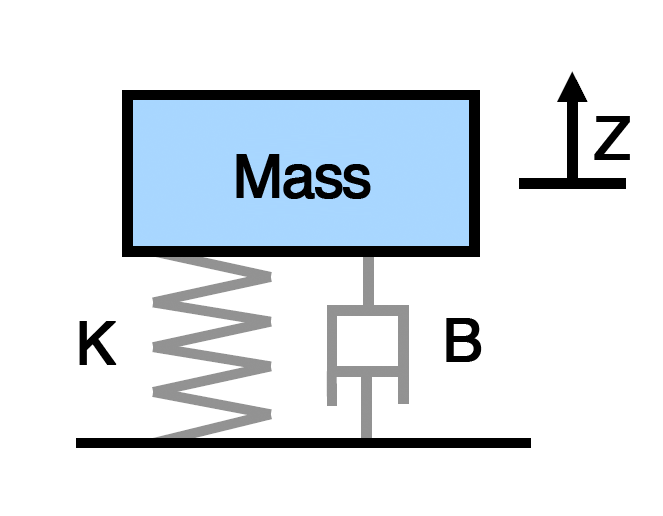
\includegraphics[width=100mm]{fig/ch4/springdamper.png}
	\end{center}
  \caption{System diagram of spring-damper contact model used in dynamic simulations.}
\end{figure}

One challenging aspect of dynamic simulations is to accurately model the effects of external forces on the system during the stance phase. To emulate the ground reaction forces during this period of the gait cycle, a contact model is used to generate an approximation of the contact force. For the purposes of this project, a simple spring-and-damper contact model is used. For the sake of simplicity, both feet of the biped are modelled as point contacts which experience a normal force proportional to the output given by Equation \ref{eq:contactf} when in contact with the ground. 

\begin{equation}
	\label{eq:contactf}
	\vec{F}_{contact} = B\vec{\dot{x}} + K\vec{x}
\end{equation}


To incorporate the effects of the contact model into the existing dynamic model, the contact force as described in Equation \ref{eq:contactf} is injected into the RNE algorithm between the end of the first pass and the start of the second pass. In other words, at the beginning of the second pass the external force used as an initial condition is modified to equal the amount of force produced by the spring damper model. Due to the serial nature of RNE, this force traverses up the kinematic chains for each leg and is finally resolved at the base. Alternatively, the equivalent force can be substituted into the overall system dynamics represented in Equation \ref{eq:motion2} for $F_{left}$ and $F_{right}$. Both approaches will yield identical results as the force is resolved into different parts of the biped robot. 

% section contact_modelling (end)

\subsection{Kajita's Matlab Toolbox} % (fold)
\label{sec:kajita_s_matlab_toolbox}
A quick and easy tool for setting up the dynamic simulations was to use an existing robotics toolbox in Matlab. Professor Shuuji Kajita packages a simple Matlab toolbox along with his textbook on humanoid robotics which provided a platform to get started with setting up the dynamic models \cite{kajitatxt}. 

\begin{figure}[!ht]
	\begin{center}
    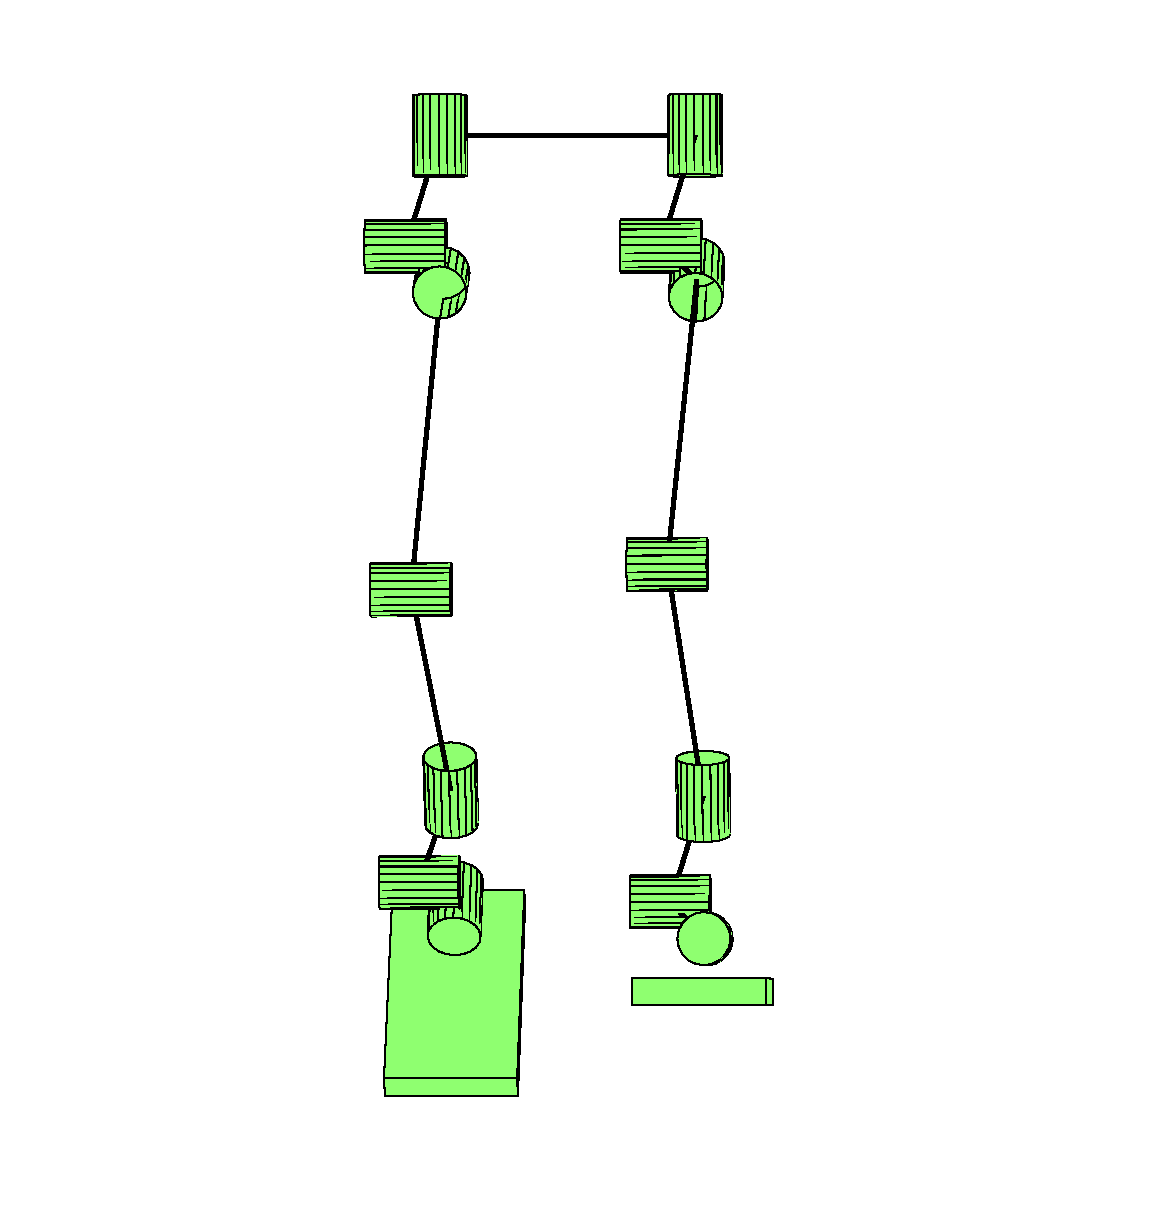
\includegraphics[scale=0.6]{fig/ch4/ulinkdrawn.eps}
	\end{center}
  \caption{Screenshot of robot structure drawn from uLINK definition.}
\end{figure}

The Matlab toolbox provides a series of scripts and functions which perform standard operations on a robotic structure (i.e. forward or inverse kinematics). Each of the functions in the toolbox revolve around the use of an object definition of the robot structure known as \texttt{uLINK}. The kinematic description for each of the links in the robot are defined as part of this \texttt{uLINK} structure using a convention specified in the accompanying textbook. An external application was written in Microsoft's .NET environment which interfaced with the API for the 3D CAD package (SolidWorks) in order to automatically generate the corresponding \texttt{uLINK} representation in Matlab code. 

Once the \texttt{uLINK} structure is established, any of the preprogrammed routines in the toolbox can be used to manipulate the kinematic structure. The most important functionality bundled with the toolbox is the direct dynamics routine. This is simply an implementation of the RNE algorithm described in Section \ref{sub:recursive_newton_euler}. However, in its original implementation the direct dynamics omits athe effects of any external forces which is necessary for the stance phase of the gait cycle. Therefore several modifications were required in order to emulate the effect of ground reaction forces through a contact model to properly size electromechanical components to withstand the impacts. 

While the toolbox provides a stable starting platform for setting up the dynamic simulation, several modifications were required in order to incorporate the effects of a contact model. The key modification required was to implement the effect of contact forces experienced by the stance leg throughout the gait cycle. Since the direct dynamics calculations were performed was based on the RNE algorithm, the modification was fairly straight forward. The initialization phase of the backwards pass in the routine (from the end of the serial kinematic chains back up to the base link) was modified according to the following code: 

\lstinputlisting{code/kajitamod.m}

Where the variables \texttt{Kr} and \texttt{Br} represent the spring and damper coefficients in the spring-damper contact model. \texttt{RCONTACT} is simply a constant link number representing the point contact foot. The velocity due to the point foot coming in contact with the ground (\texttt{vr}) is recomputed by considering the original velocity (\texttt{vo}) and the cross product between the position of the foot (\texttt{uLINK.p}) and angular velocity (\texttt{uLINK.w}). The resulting normal force is computed and injected into the backwards pass if the foot position is below the ground level (condition shown in line 1). 

Using this conditioning, the initialization sequence of the backwards chain simply checks for the position of each foot in world coordinates to determine whether ground contact is present. The ground throughout the simulation is assumed to be represented by the $z = 0$ plane. Therefore, for any value of $z > 0$ the foot is not in contact with the ground and subsequently $z \leq 0$ represents contact is present. In the situation where contact is present, a ground normal force proportional to the output of the spring-damper system is injected into the system. Due to the recursive nature of the RNE algorithm, this force back-propagates through each of the links in the serial chain until it is ultimately resolved at the terminating base link.
% subsection modifications (end)

% section kajita_s_matlab_toolbox (end)

\subsection{Gait Estimation} % (fold)
\label{sec:gait_estimation}
	
In order to emulate the operating conditions for the lower body biped robot once it is built, the dynamic simulation must incorporate the effects of executing a gait cycle. This allows for investigation into the external  forces experienced by the robot structure while walking. 
	
One method of emulating the normal operating conditions is to estimate the effects by using human gait. While it is highly ambitious that a walking robot will be able to achieve the performance of human-like walking, it provides a basis to from which the initial selection of electromechanical components can emerge. The goal is to extract the kinematic parameters experienced by the human limbs while walking and impose similar conditions in the dynamic simulation. Given these constraints, the inverse dynamics problem can be solved in order to obtain the joint torque estimates during various points in the gait cycle. Coupled with the modifications to emulate contact forces during the stance phase, this simple dynamic simulation provides a quick and easy way to estimate the torque loading at the joints to develop initial design specifications. 
	
In order to use kinematic parameters from human gait, data published from the 2008 Dynamic Walking conference was used \cite{dw2008}. The published data used several sensors to measure the joint angles and velocities of lower body human limbs under several gait cycle speeds (i.e. fast walk, slow walk, normal walk, etc). During the data collection, sensors were strategically placed such that key information such as the knee yaw and hip pitch was captured. This raw sensory data was imported into the Matlab environment using a 3D motion analysis toolbox known as BodyMech \cite{bodymech}. This information was incorporated into the dynamic simulation by enforcing the joint angles, velocities and accelerations from each captured frame of the reference dataset. By accomplishing this, the \texttt{uLINK} robot structure which modelled the dynamic parameters (mass, link inertias) with the captured 3D kinematics of human gait. 

An experiment was devised in the Matlab environment which used a combination of the BodyMech toolbox and Kajita's toolbox. The BodyMech toolbox was used to extract the frame-by-frame 3D kinematic parameters as a human executed the gait cycle. These parameters were processed and stored in order to be played back on the robot model defined by the \texttt{uLINK} structure. The Matlab script provided in Appendix \ref{sec:gait_analysis_script} was used to load the 3D kinematic parameters from each frame and apply the transformed equivalent on the robot structure. To compensate for the differences in size between humans and the small biped, the joint velocities and accelerations were scaled by selecting a different reference gait speed from the published data set. 
	
Once the parameters were applied, the inverse dynamics routine was executed in order to determine the torques at each joint in the structure as result of the gait dynamics. Note that the inverse dynamics routine was also modified to emulate the contact force effects experienced during the stance phase of the gait cycle. This process was repeated for each frame in the captured data and the results of robots kinematics and dynamics ($q$, $\dot{q}$, $\ddot{q}$ and $\tau$) were tabulated in CSV files for post processing. 
	
\begin{figure}[!ht]
	\begin{center}
	\begin{tabular}{cc}
	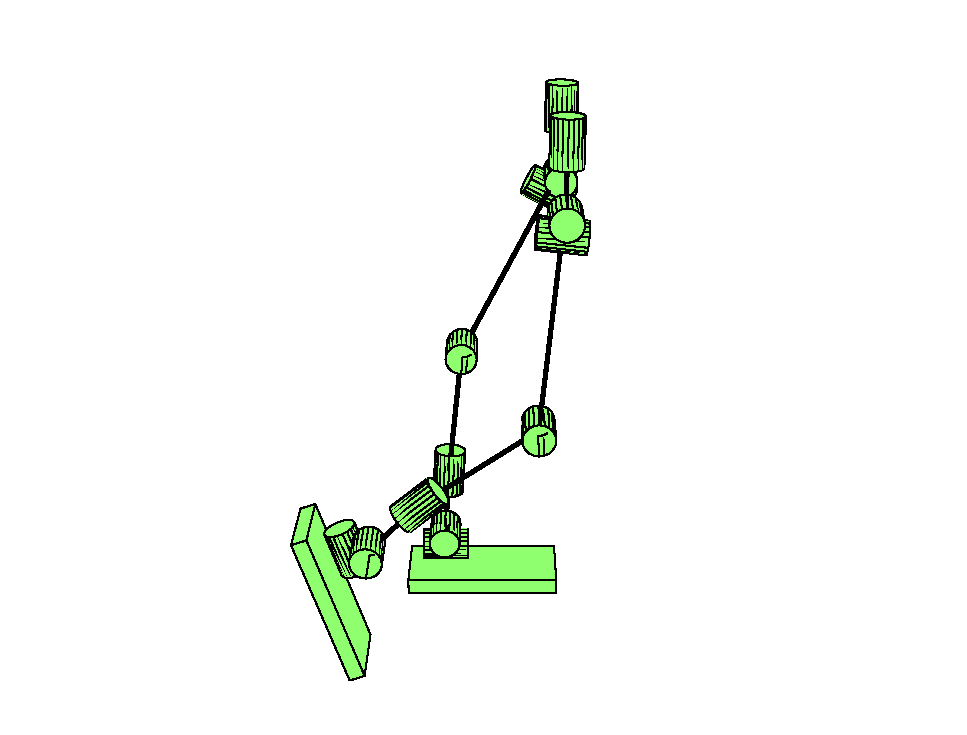
\includegraphics[scale=0.5]{fig/ch4/ulinkwalk1.eps} &
    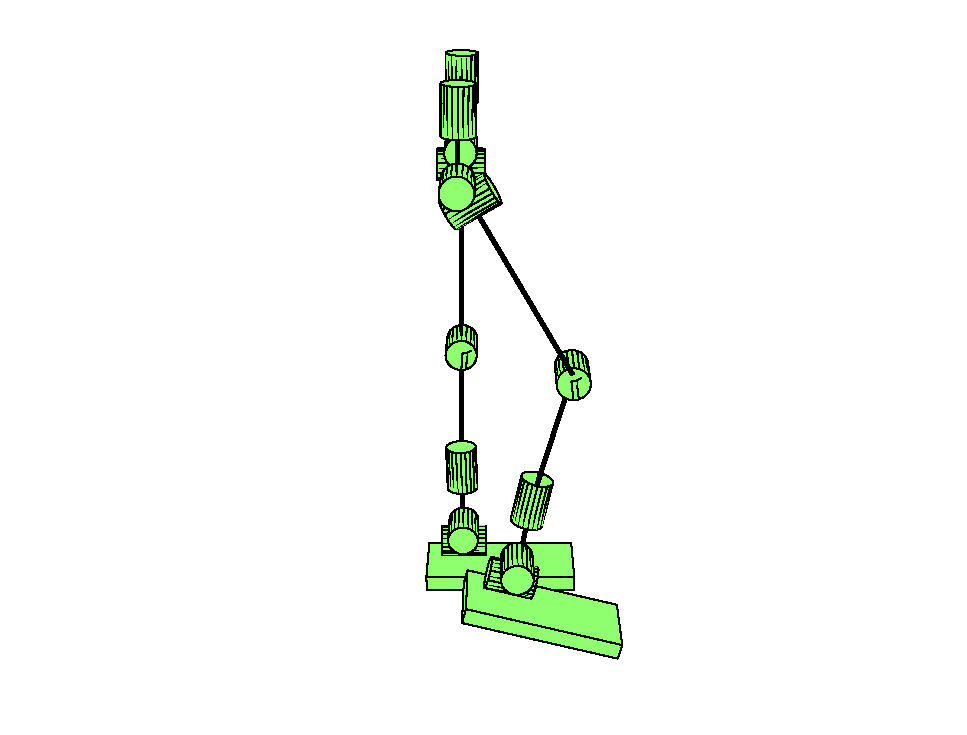
\includegraphics[scale=0.5]{fig/ch4/ulinkwalk.eps}
	\end{tabular}
	\end{center}
  \caption{Screenshot of gait analysis of uLink structure executing human-walk.}
\end{figure}
	
% section gait_estimation (end)


\subsection{Initial Design Requirements} % (fold)
\label{sec:initial_design_requirements}

\begin{figure}[!ht]
	\label{fig:gaitplot}
	\begin{center}
    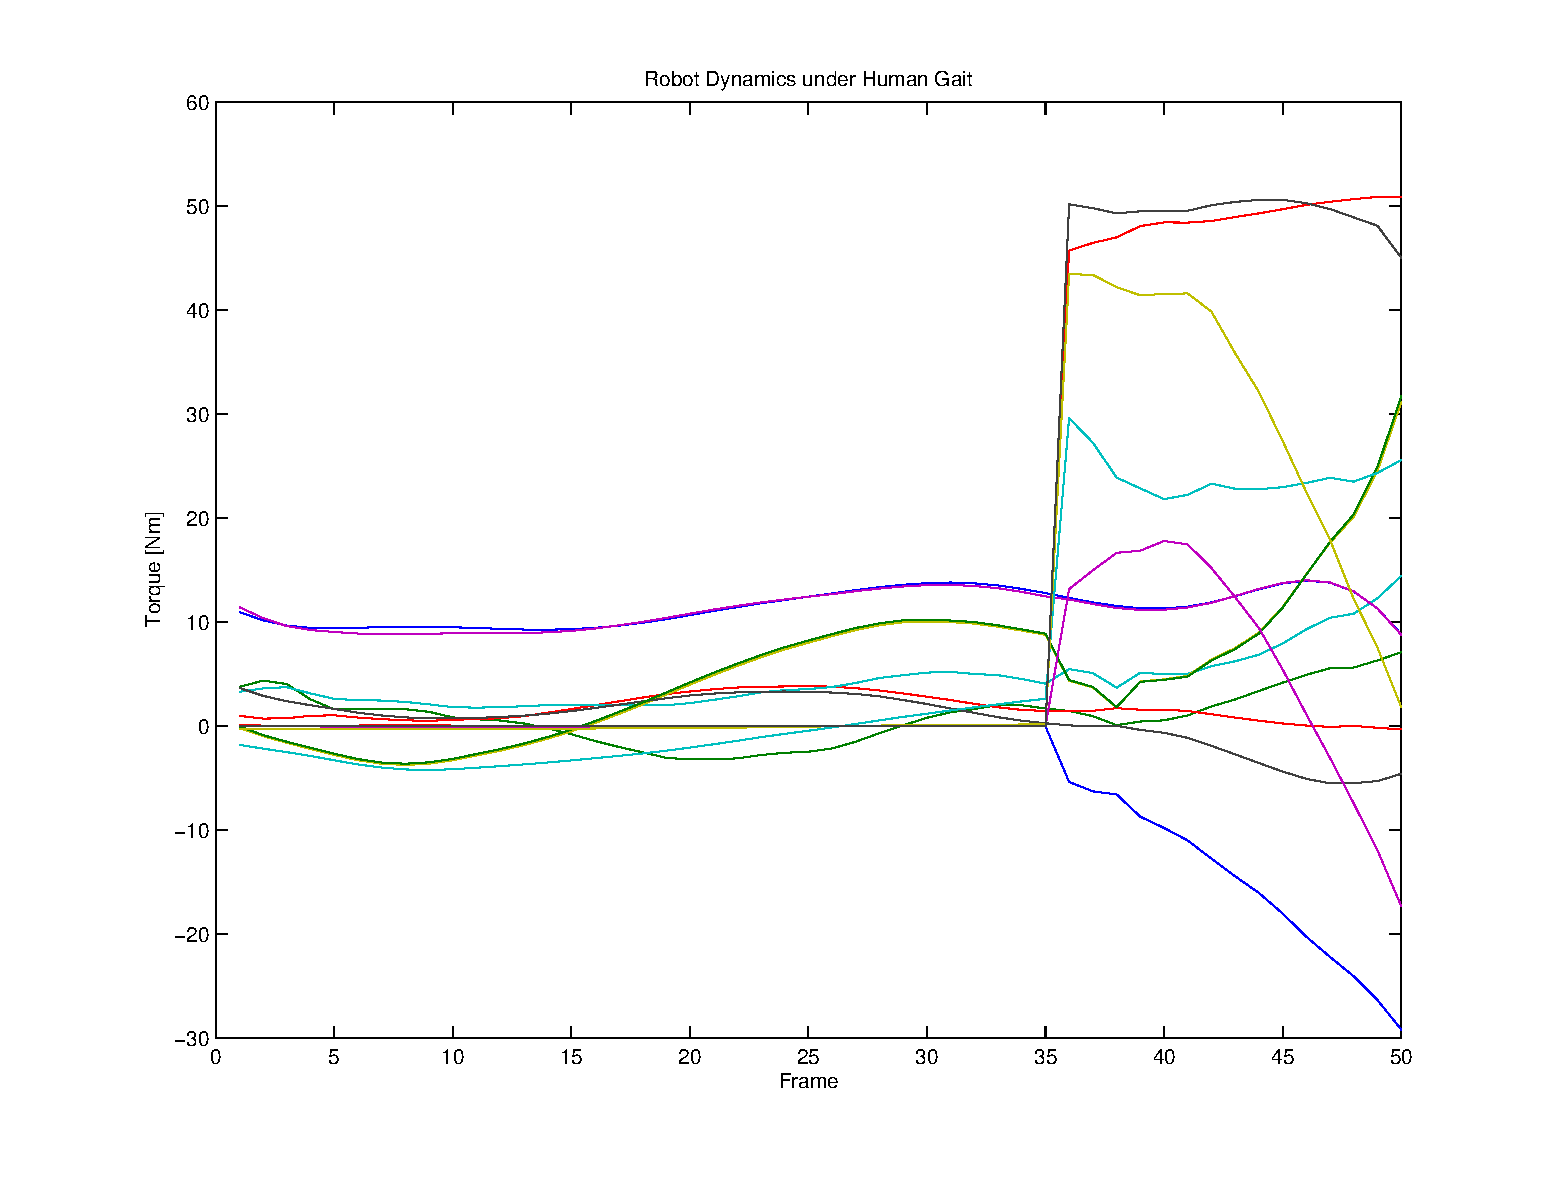
\includegraphics[scale=0.6]{fig/ch4/gaitplot.eps}
	\end{center}
  \caption{Joint torque profile during the execution of human-gait kinematics from reference data set.}
\end{figure}

The results of the dynamic simulations under human-gait analysis form the basis for the initial electromechanical components selection process. As expected, it was observed that the largest demands in torque loading on each of the joints occurred during the stance phase immediately after the heel strike event (refer to Frame 36 in Figure \ref{fig:gaitplot}). The torque demands at that instant spike immediately to almost 3x the steady state torque loading on the joints. While it is expected that a walking robot will experience large spikes in the torque demands such as the ones observed in the dynamic simulation, it is unreasonable to use only the peak torque values as the required specifications for design. 

\begin{table}[!ht]
  \centering
  \caption{Individual joint torque demands for each DOF in one leg.}
    \begin{tabular}{lcc}
    \addlinespace
    \toprule
    \textbf{Joint} & \textbf{Normal} & \textbf{Peak}\\
    \midrule
    Ankle Roll	&	13.824 Nm	&	14.021 Nm\\
    Ankle Pitch	&	4.395 Nm	&	7.923 Nm\\
	Ankle Yaw	&	3.858 Nm	&	3.858 Nm\\
	Knee Pitch  &	5.229 Nm	&	16.539 Nm\\
	Hip Roll	&	13.606 Nm	&	14.054 Nm\\
	Hip Pitch	&	10.081 Nm	&	38.295 Nm\\
	Hip Yaw		&	3.698 Nm	&	3.698 Nm\\
    \bottomrule
    \end{tabular}%
  \label{jointtable}%
\end{table}%


Since one of the secondary objectives is to keep the overall mass of the biped as low as possible, it is desirable to select smaller motors where the peak torque loading on the joints are outside of the allowable range of continuous operation. This is a reasonable estimate since the peaks are impulsive forces which only last for a short period of time. The practical approach for deriving specifications from the dynamic simulations is to analyze the continuous torque loading while the system undergoes the gait cycle while keeping the peak loading requirements as a secondary objective. 

While the torque demands vary from one joint to the next (see Table \ref{jointtable}), the results from the analysis are concatenated to obtain only a single set of design specifications. This also helps to limit the different types of motors selected from the manufacturer and greatly simplifies the electromechanical design process. The task of fine tuning the motor selection for each joint is left for future revisions. Therefore, the set of design specifications for the joint torques are summarized in Table \ref{tab:spectable}

\begin{table}[!ht]
  \centering
  \caption{Initial design specifications for electromechanical components.}
    \begin{tabular}{lcc}
    \addlinespace
    \toprule
    \textbf{Condition} & \textbf{Torque} & \textbf{Velocity}\\
    \midrule
    Normal & 14 Nm & 2.48 rad/s\\
    Peak  & 50 Nm & 6.82 rad/s \\
    \bottomrule
    \end{tabular}%
  \label{tab:spectable}%
\end{table}%

For the initial design consideration, the normal torque specification shown in Table \ref{tab:spectable} is obtained by taking an average of joint torque values during the swing phase. Since the ground reaction forces experienced during the stance phase produce large torques in a short period of time, the peak torque specification in Table \ref{tab:spectable} is obtained by selecting the highest torque value from all frames.

The contact model parameters (spring and damping coefficients) were observed to have a noticeable effect on the peak design specifications. Since the contact model only provides a crude approximation of the ground reaction forces that the real robot will experience, the final selected value was chosen to provide a peak torque which averages between the largest and smallest values. The final spring and damping coefficients used in deriving the design specifications were $K = 10000$ and $B = 100$, respectively.
% section chassis (end)


%======================================================================
%   D R I V E T R A I N  S E L E C T I O N
%======================================================================


\section{Drivetrain Selection} % (fold)
\label{sec:drivetrain}
Lorem ipsum dolor sit amet, consectetur adipisicing elit, sed do eiusmod
tempor incididunt ut labore et dolore magna aliqua. Ut enim ad minim veniam,
quis nostrud exercitation ullamco laboris nisi ut aliquip ex ea commodo
consequat. Duis aute irure dolor in reprehenderit in voluptate velit esse
cillum dolore eu fugiat nulla pariatur. Excepteur sint occaecat cupidatat non
proident, sunt in culpa qui officia deserunt mollit anim id est laborum.
% section drivetrain (end)

% chapter design (end)
    \chapter[Toolchain Development]{Toolchain Development\footnote{A version of this chapter has been accepted for publication at the 2012 IEEE International Conference on Humanoid Robots \cite{ChoudhuryHumanoids2012}}} % (fold)
\label{cha:toolchain}

This chapter introduces a rapid prototyping toolchain\footnote{This work was completed in collaboration with Quanser Inc through the Natural Sciences and Engineering Research Council (NSERC)'s Industrial Postgraduate Scholarship Program.} developed to streamline the process of exporting a prototype design from a CAD software package to generate dynamic simulations with full 3D visualization. Starting from the initial prototype design and drivetrain specifications in the previous chapter, the design process outlined in Section~\ref{sec:design_process} is used to improve the overall system performance. The toolchain provides an automated two-step process which begins by exporting key information from CAD (Section~\ref{sec:cad_export}) and ends by regenerating the equivalent system in a simulation environment (Section~\ref{sec:model_generation}). A case study is presented in Section~\ref{sec:case_study} demonstrating the performance benefits of the proposed toolset. 

The electromechanical design and development of multibody robotic systems is an iterative process, starting from a mechanical model in CAD software, transferring its parameters to a dynamic simulator for analysis and revising the design to improve the performance of the system. This process is repeated until the mechanical design achieves some desired goal. The iterative nature of the design and analysis process can often become time consuming and cumbersome. However, for high DOF multibody systems, the iterative approach is necessary as small changes in the mechanical design can have a significant impact on the overall dynamics of the system and the resulting system behaviour as well as implications for control design. Another popular approach is the use of optimization tools \cite{Paul2001,Wollherr2002} to determine the optimum design configuration. However, the resulting configuration may not be realizable with the available hardware components and must still be verified in simulation before hardware implementation. Ravichandran et al. used a hybrid evolutionary algorithm which optimizes discrete (e.g. available actuators) and continuous (e.g. link lengths) design variables to obtain the optimum design configuration which is realizable with commercial off-the-shelf parts \cite{Ravichandran:2004}. This approach optimizes the design for \emph{specific} tasks with predefined trajectories, which may be impossible to define for some multibody robotic systems with complex applications (i.e. bipedal robots with on-line gait generation). 

\section{Design Process} % (fold)
\label{sec:design_process}

The initial prototype design process of the 14 DOF bipedal robot presented in Chapter~\ref{cha:design} illustrates the need for a streamlined toolchain. Prior to obtaining the initial torque estimates from dynamics simulations, a basic bare-bones mechanical model of the bipedal robot was constructed in CAD (with $n = 14$ joints and $m = n+1 = 15$ links). This initial mechanical model included arbitrary DC motor models from the manufacturer since the torque required was yet to be determined. After executing the dynamic simulations using Kajita's toolbox for the first time, the torque estimates were used to revise the mechanical design in CAD with more appropriate motors. However, this design revision altered the robot dynamics (e.g. increased mass due to larger motors) which effects the joint torques required to support the updated mechanical model during the estimated gait cycle. The design process of executing the dynamic simulations, obtaining updated torque estimates and revising the mechanical model with more appropriate motors was repeated several times. The process ended once a suitable motor configuration capable of producing the estimated torque required its own mechanical model was found. The frequent and incremental design revisions required moving back and forth between the CAD software package and the dynamic simulation environment. Each design revision required transferring the updated kinematic and dynamic parameters of the links back to the simulation environment prior to executing the simulation. 

There exists a wide variety of dynamic simulation environments with a range of capabilities \cite{Koenig04designand,michel2004webotstm, Kanehiro:2004dq, PonticelliCWR2006, Reichenbach2009, MedranoCerda2010}. These environments provide a feature-complete package, which combine an underlying dynamics engine with an interface for visualizing the simulations. The underlying computation engines obtain the complete equations of motion for the system described by its kinematic/dynamic parameters using techniques including, but not limited to, Lagrange multipliers \cite{Baraff1996}, Kane's method \cite{Rosenthal1986} and port-based modeling \cite{Paredis2001}. The equations of motion are integrated to obtain the system state at each time step. Most simulators provide support for importing common Virtual Reality Markup Language (VRML) or Standard Tessellation Library (STL) files generated by CAD tools for visualization \cite{Koenig04designand,michel2004webotstm}. However, only a few provide direct compatibility with CAD tools to import kinematic/dynamic parameters for simulation.

Open Architecture Humanoid Robotics Platform (OpenHRP) \cite{Kanehiro:2004dq} is a commonly used dynamic simulation environment for humanoid robots that supports importing VRML files. However, kinematic and dynamic parameters of the robot are specified as plain text, making it cumbersome for rapid iterations.

MapleSim \cite{sw:maplesim} is a multibody simulation package that provides limited functionality to communicate with CAD applications through its MapleSimConnector toolbox. This toolbox uses the underlying Maple engine with command-line access for retrieving the parameters of each link. However, the CAD application has to be actively running in the background and it is left to the user to generate Maple worksheets for batch importing of the parameters to update the link parameters in MapleSim through its API.

SimMechanics \cite{sw:simmech} provides mechanical import functionality to generate Extensible Markup Language (XML) files containing link parameters directly from CAD along with the corresponding STL files for visualization. However, there are limitations on how joint constraints are defined in CAD to successfully generate an equivalent model in Simulink. Another drawback of this approach is that the visualization generated during simulations significantly impacts the simulation speed.
% section design_process (end)

\section{CAD Export} % (fold)
\label{sec:cad_export}

An add-in was developed for CAD software package SolidWorks to export a multibody system for dynamic simulations in Simulink with realtime visualization. Consider a standard multibody system with $n$ joints and $n + 1$ links. The links are numbered from 0 (base) to $n$ and each $joint_{i}$ connects $link_{i-1}$ to $link_{i}$. The mechanical design of each link is represented by its own CAD assembly (or part) file. The coordinate system at the origin of this CAD file is treated as the local coordinate system $xyz_{i}$ rigidly attached to the link $i$. The top-most CAD assembly (referred to as the \emph{master assembly}) contains all $n + 1$ links as subassembly files connected and constrained by the mechanical relationship which defines the behaviour of each joint $n$. For example, a revolute joint connecting two link subassemblies is defined by the appropriate constraints (e.g. concentric relationship).

\begin{figure}[!h]
	\centering
    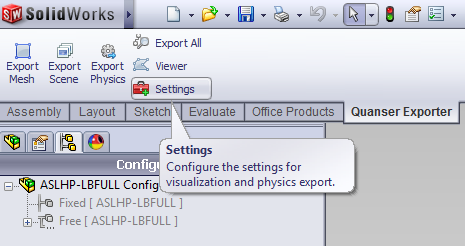
\includegraphics[scale=1.0]{fig/toolchain/exporter.png}
  	\caption{The exporter add-in for SolidWorks (named Quanser Exporter in the SolidWorks tab) to capture relevant physical and visualization data.}
	\label{fig:swexporter}
\end{figure}

The add-in for SolidWorks uses this master assembly file as a starting point to export the multibody system for dynamic simulations. Once installed, a new tab is added directly in SolidWorks (as shown in Figure~\ref{fig:swexporter}) presenting the user with several export options. The initial export process prompts the user with a flat list of all subassemblies in the current file via a \emph{Model Organizer} interface (shown in Figure~\ref{fig:modelorg}). Each subassembly is treated as a node that can be ordered (through a drag-and-drop interface) to form the desired kinematic tree/chain hierarchy. 


\begin{figure}[!h]
	\centering
    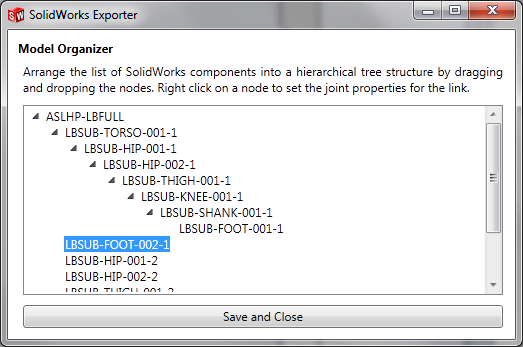
\includegraphics[scale=1.0]{fig/toolchain/modelorg.png}
  	\caption{The \emph{Model Organizer} window used to define the kinematic hierarchy of links during initial export.}
	\label{fig:modelorg}
\end{figure}

\subsection{Physics Export} % (fold)
\label{sub:physics_export}
Each link subassembly is parsed in the order defined in the \emph{Model Organizer} window to extract key kinematic/dynamic parameters. All numerical values (e.g. distance between links) are extracted directly using CAD tools. Assuming that the system is in the home configuration at the time of export, the relative frame transformations $T^{i-1}_{i}$  between subsequent frames are extracted in accordance with the kinematic hierarchy defined in the \emph{Model Organizer}. The absolute frame transformations $T^{0}_{i}$ are also computed with respect to the base link (if the base link is fixed in the master assembly file). For floating base systems (i.e. base link has 6 DOF), the absolute frame transformations $T^{W}_{i}$ are taken with respect to the coordinate system of the master assembly file (world frame). The mass and dynamic properties are extracted with internal CAD tools in the local coordinate system of the link subassembly file. The mass, distance to the center-of-mass (COM) and inertia tensor of the link (at the COM position) are extracted.

The add-in captures these key parameters and generates a structured XML file. An XML node is generated for each link containing the extracted kinematic/dynamic parameters (as shown in Figure \ref{fig:exportfile}). Furthermore, each XML link node is organized in accordance with the kinematic hierarchy of the system. As a result, the add-in captures the entire physical description of the multibody system in a portable, language-independent file.

\begin{figure}[!h]
	\centering
    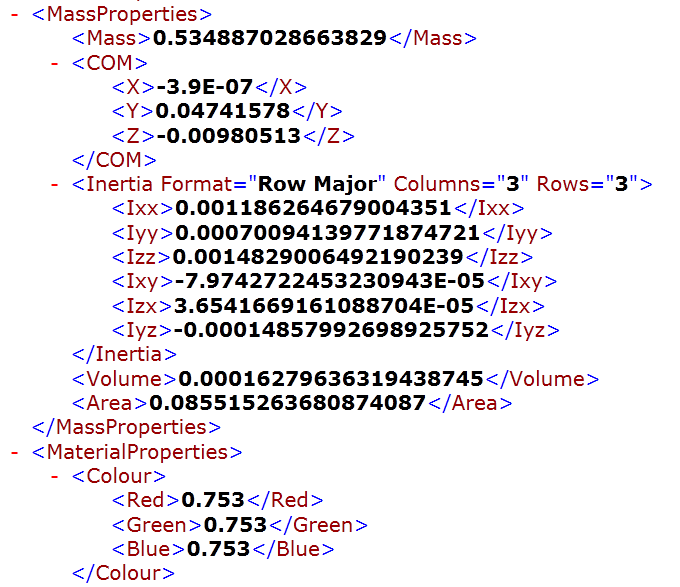
\includegraphics[scale=0.6]{fig/toolchain/exportfile.png}
  	\caption{Example of kinematic and dynamic parameter extraction straight from CAD model stored in the exported XML file.}
	\label{fig:exportfile}
\end{figure}

% subsection physics_export (end)

\subsection{Mesh/Scene Export} % (fold)
\label{sub:mesh_scene_export}
In addition to exporting the physical description of the model, the exporter add-in also generates files for visualization. These files can be used in conjunction with dynamic simulations to provide the user with visual feedback of the system under control. Some dynamic simulators (SimMechanics, MapleSim) currently allow users to specify a VRML file for each component of the multibody system. While SolidWorks currently has some support to export VRML files for each link subassembly individually, there are no options to generate the 3D meshes in X3D format (successor to VRML).

The toolchain provides automatic batch generation of full 3D meshes in the X3D format for each link subassembly. Once the export process has been initiated, the meshes are extracted for each link subassembly in the master assembly file directly from the CAD layout. Figure~\ref{fig:meshfile} shows the X3D mesh generated from a link subassembly in CAD. Each mesh is aligned with the local coordinate system of the link such that there is a direct mapping between the visualization and the physical model.

\begin{figure}[!h]
	\centering
    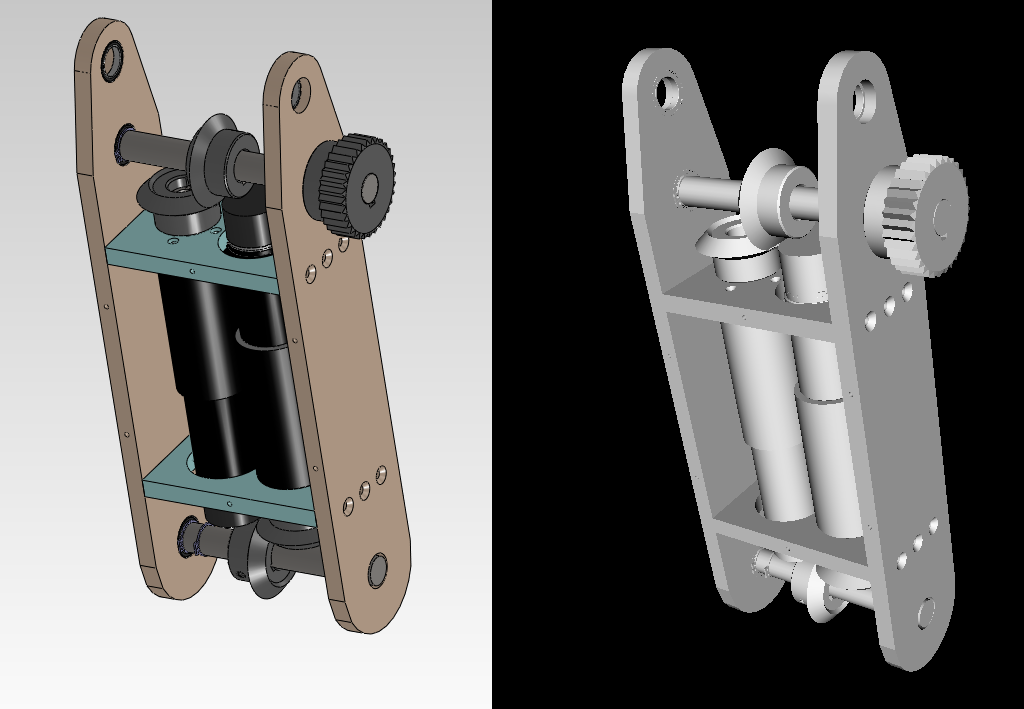
\includegraphics[scale=0.5]{fig/toolchain/cad2x3d.png}
  	\caption{Equivalent X3D mesh file (shown on the right) generated directly from CAD layout (shown on the left) for a single link subassembly.}
	\label{fig:meshfile}
\end{figure}

The overall mesh generation process is optimized for complex multibody systems. A typical CAD subassembly representing each link may contain hundreds of smaller CAD part/assembly files. During the mesh generation process the add-in creates a new flattened version of each link subassembly and discards any visual details not visible on the surface. The surfaces of this flattened model are tessellated to generate the mesh file for each link. As a result, the mesh files are light weight and this helps speed up the rendering process.

The output mesh files are stored in the same directory as the XML file containing the physical description of the system. Furthermore, each link XML node is also updated with a complete path to its corresponding mesh file alongside the kinematic/dynamic parameters. The add-in also generates a \emph{scene} file from the CAD master assembly. This is a parallel XML file which contains a complete visual description of the system from CAD. The scene file contains a list of all links alongside their corresponding mesh files. These meshes are then organized in accordance with the kinematic tree/chain hierarchy provided by the user in the \emph{Model Organizer}.

As a result, the scene file recreates the visual layout of the complete multibody system from the CAD master assembly file. This file encapsulates the full multibody system in a format which is compatible with the 3D visualization blocks that are packaged with the QUARC toolbox. In addition to the model itself, additional supplementary mesh files (e.g. ground plane) are imported into the scene for visualizing the environment.
% subsection mesh_and_scene_export (end)

\subsection{CAD Update} % (fold)
\label{sub:cad_update}
With minimal user input, the add-in captures a complete physical and visual description of the system in its \emph{current state}. However, the main benefit of this toolchain becomes apparent after the initial export. Once the user defines the structure of the system (kinematic hierarchy and joint definitions) through the \emph{Model Organizer}, it is stored in memory for later use. Subsequent updates to the CAD model can be exported with a single click if the overall structure of the links and joint definitions do not change.

This allows the user to export a model for simulation from CAD, analyze the behaviour of the system under control, tweak the mechanical design and immediately re-export the revised model for simulation. For example, increasing the length of a link may alter its dynamic properties  while the overall kinematic structure remains the same. The revised CAD model with increased link length can be exported with a single click. The export process simply recalls the structure of the system and regenerates the XML files with updated kinematic/dynamic properties. The add-in also allows the user to regenerate only the mesh file for the updated link to reflect the changes in CAD. This process makes it fast and easy for rapid iterations during the design phase.
% subsection cad_update (end)

% section cad_export (end)

\section{Model Generation} % (fold)
\label{sec:model_generation}

The XML files exported by the add-in encapsulate the relevant CAD model information into structured and portable files. One of the key advantages of this approach is that the information in these files can easily be parsed to generate an equivalent model in most dynamic simulators. A model generation counterpart was developed for the Matlab/Simulink environment which uses SimMechanics for multibody dynamic simulation and Quanser's QUARC toolbox for 3D visualization. This provides a semi-automated toolchain for designing robotics and/or mechatronic systems.

The model generation approach provides several Matlab functions, scripts and libraries to parse the files exported by the SolidWorks add-in and generate the equivalent mechanical system in Simulink. The generated Simulink model contains (a) SimMechanics blocks with the link kinematic and dynamic parameters from CAD and (b) visualization blocks from QUARC libraries with the link meshes and scene file. The generated physics and visualization counterpart is pre-populated with CAD data and connected according to the kinematic hierarchy of the system defined in the \emph{Model Organizer}.

The model generation process is initiated by calling a function in the Matlab terminal inside the CAD export folder. By default, this approach generates a physical subsystem (i.e. the “plant”) for forward dynamics simulation, whose output drives a generated visualization subsystem. The user can also generate an inverse dynamics model through the command line.

\subsection{Physical Model} % (fold)
\label{sub:physical_model}

The physical model generation process parses the XML output files in the export folder to create a CAD-equivalent system in Simulink. In order to streamline the process, a library of masked link subsystems representing common link configurations (shown in Figure \ref{fig:quarcmech}) was developed. Each of these subsystems contains a combination of SimMechanics joint, body, actuator and sensor blocks to represent a combination of $joint_{i}$ and $link_{i}$ (shown in Figure \ref{fig:undermask}).

\begin{figure}[!h]
	\centering
    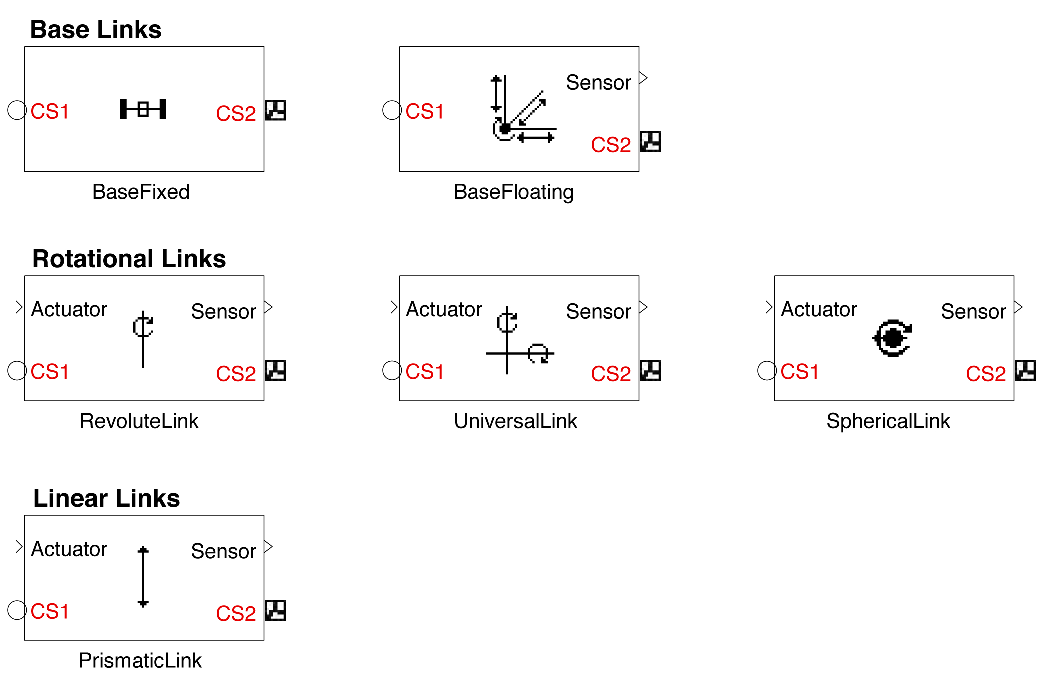
\includegraphics[scale=0.75]{fig/toolchain/simmech.pdf}
  	\caption{The standard link subsystems for physical model generation with prepopulated kinematic and dynamic parameters from CAD.}
	\label{fig:quarcmech}
\end{figure}

The input to each link subsystem (\textbf{CS1}) is a connection from $link_{i-1}$ and the driving signal for the joint. The output of the link subsystem is its local coordinate system (\textbf{CS2}) and the joint sensor signals. The joint actuator/sensor signals are set depending on the type of dynamic simulation. By default the model generation process configures the physical model in forward dynamics mode so the joint actuator port is connected to the force/torque command input for $joint_{i}$ and joint angle/displacement is measured at the output. Alternatively, for the inverse dynamics simulation, the joint acceleration is set as the input, while the joint force/torque is the output. The output coordinate system of the $joint_{i}$ block is connected to a SimMechanics body block representing $link_{i}$. The masked parameters are preconfigured to set the local dynamic properties (e.g. COM position, inertia tensor) and relative frame transformation appropriately.

\begin{figure}[!h]
	\centering
    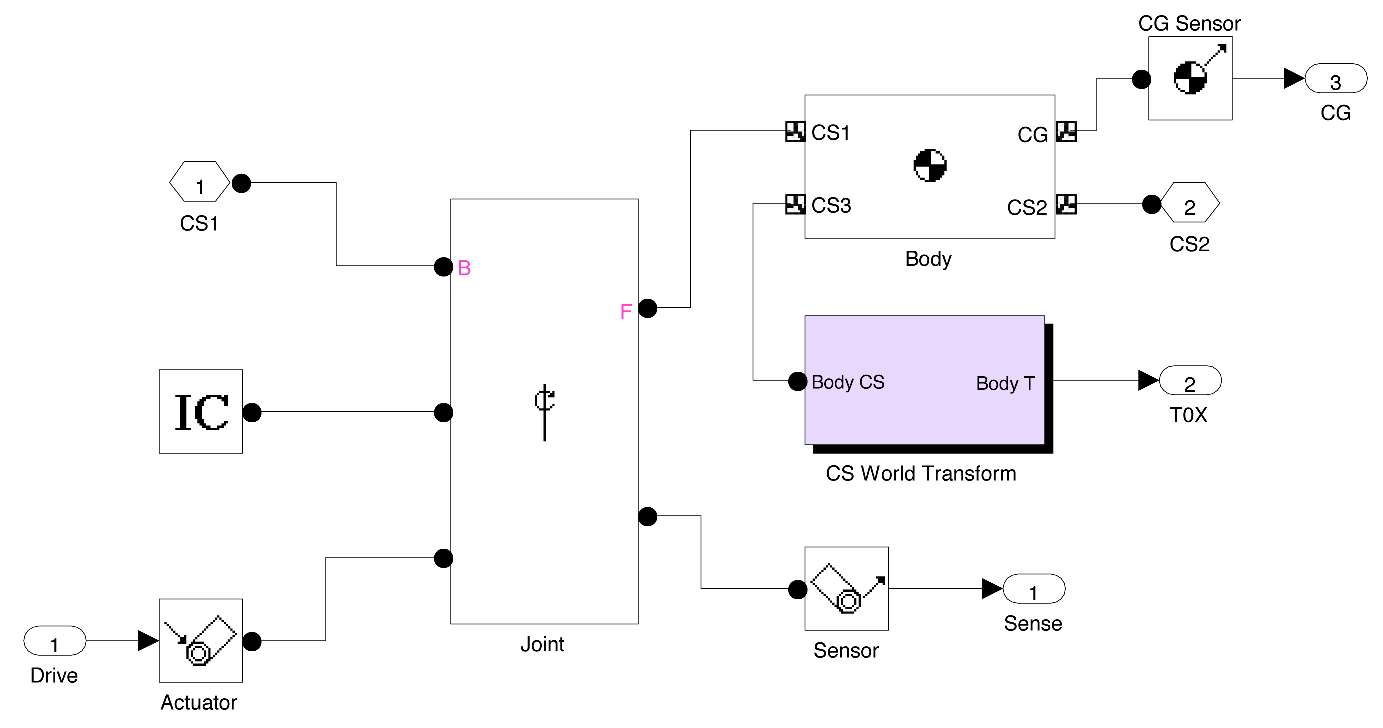
\includegraphics[scale=0.6]{fig/toolchain/undermask.pdf}
  	\caption{SimMechanics blocks used to compose each CAD-equivalent link subassembly in Simulink}
	\label{fig:undermask}
\end{figure}

Each link subassembly from CAD is recreated with a link subsystem from the library depending on the link type. The masked parameters are populated with the kinematic and dynamic parameters from the corresponding XML link node. The overall hierarchy of links is parsed and each link subsystem is connected accordingly. The model generation process also automatically handles the signal routing from the input/output ports of the physical model. In the default forward dynamics configuration, the $n \times 1$ torque/force vector is connected to all joint actuator blocks and the output signals from the sensors are also routed accordingly. For the inverse dynamics case, the vector of joint positions, velocities and accelerations are connected to the joint actuator blocks and the sensors are preconfigured to output the resulting torque/force vector.

In addition to the link subsystem, a ground block representing the coordinate frame of the CAD master assembly is connected to the base $link_{0}$. The entire process of creating an equivalent model for dynamic simulation is automated. The user simply calls the appropriate function and the generated physical model subsystem is placed in a new (or existing) Simulink diagram.
% subsection physical_model (end)

\subsection{Visualization Model} % (fold)
\label{sub:visualization_model}
The visualization model generation process generates a single subsystem containing blocks to initialize and drive the scene file generated from CAD. The mesh for each link in the kinematic chain is driven by the output of the generated physical model (forward dynamics subsystem) so that there is a 1:1 mapping between the plant and what is being rendered by the visualization. When a simulation is running, an external 3D viewer application (part of the QUARC toolbox) is used to render the scene in real-time using OpenGL (CAD-equivalent visualization scene file shown in Figure \ref{fig:masterscene}).

\begin{figure}[!h]
	\centering
    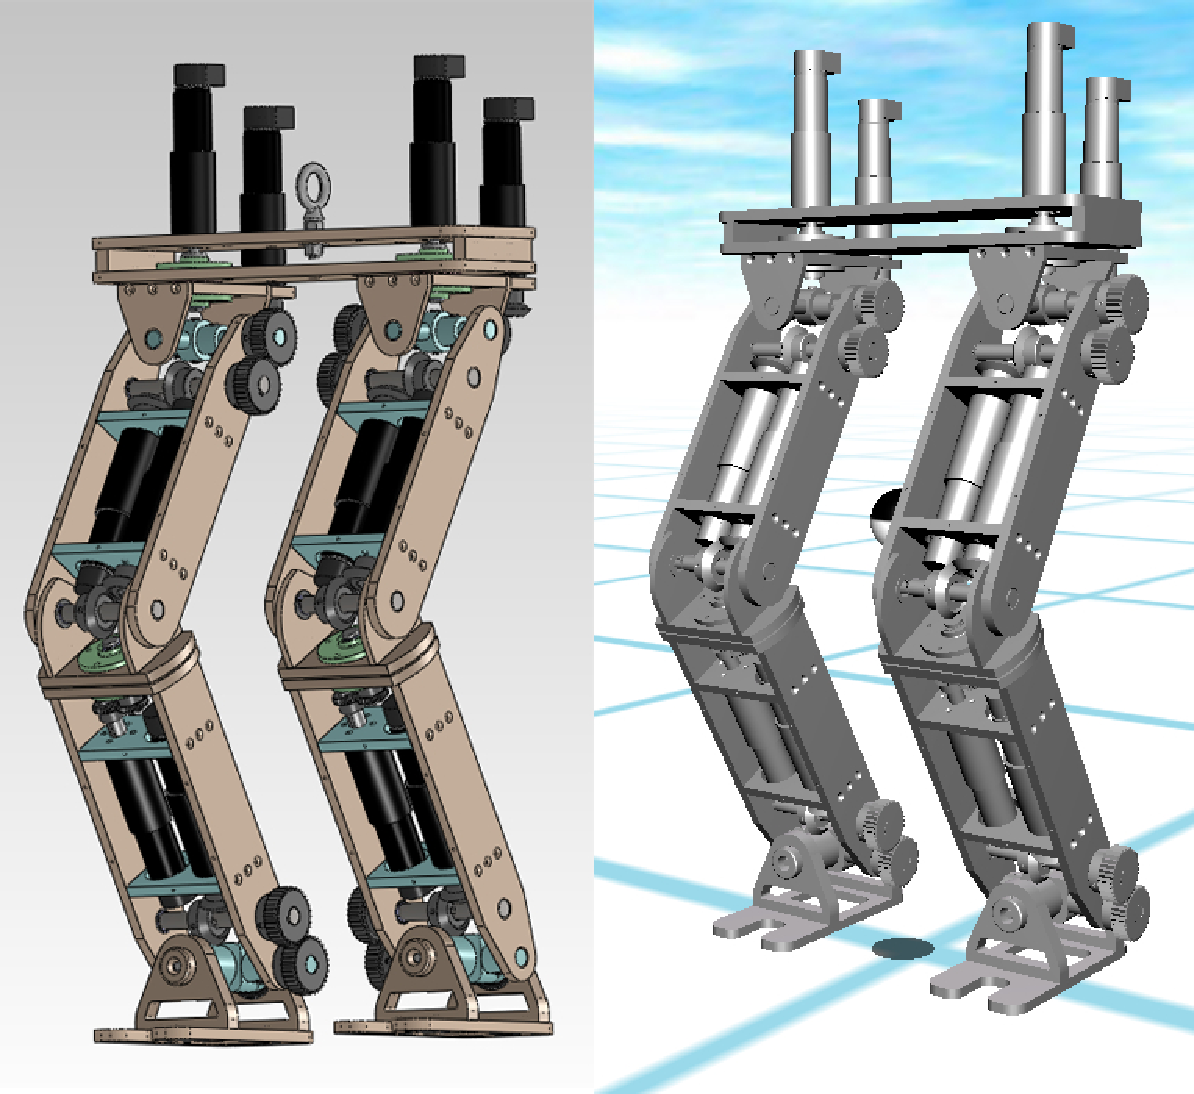
\includegraphics[scale=0.50]{fig/toolchain/masterscene.pdf}
  	\caption{CAD master assembly shown on the left is used to automatically generate the meshes and scene file to recreate the visualization shown on the right.}
	\label{fig:masterscene}
\end{figure}

This approach allows the user to receive immediate visual feedback of the CAD model under the influence of control. This also allows the user to make changes to the mechanical design from visual observations (e.g. quick changes to improve joint limits).
% subsection visualization_model (end)

\subsection{Model Update} % (fold)
\label{sub:model_update}
The exporter add-in makes it possible to make changes to the mechanical design in CAD and generate the new kinematic and dynamic parameters immediately. After the initial model generation from CAD data, these new changes can be reflected back into the dynamic simulation by simply calling the update function. The update functionality also allows the user to specify the path to the previously generated physical model. The masked parameters on each link subsystem inside this model are simply updated with the new changes while the signal routing and everything else is left intact. The updated mesh files are loaded by the QUARC 3D viewer during the next simulation run.

This streamlines the iterative design process by allowing a user to export a system from the add-in and generate the CAD-equivalent physical/visual model in Simulink. The behaviour of the system can then be analyzed in dynamic simulations to revise the CAD design. Once the new changes are applied, the revised parameters are easily exported back into dynamic simulations for further analysis.
% subsection model_update (end)

% section model_generation (end)

\section{Case Study} % (fold)
\label{sec:case_study}

This toolchain was used to improve the initial design of the 14 DOF lower body humanoid robot\footnote{A video demonstration of the toolchain being used is available online at: \\ \url{https://ece.uwaterloo.ca/~dkulic/videos/Humanoids2012-480p.mp4}} discussed in Chapter \ref{cha:design}. The toolchain was used to quickly analyze the effects of design revisions (e.g. compare motor positioning) in simulation prior to manufacturing. The complete initial export and model generation process takes about two minutes for the 14 DOF bipedal robot. Since the kinematic hierarchy and joint information is stored during the initial export process, subsequent exports take around thirty seconds to reflect the design revisions from CAD back into the dynamic simulator. 

\subsection{Dynamic Simulations} % (fold)
\label{sub:dynamic_simulations}

The proposed toolchain was used during the design phase to estimate the torques at each joints for appropriate motor sizing. Note that the mechanical design in CAD includes the selected motor models from the manufacturer. Changes to the mechanical design such as motor positioning and material of the links can significantly alter the torques required at some joints. In these situations it is useful to make incremental changes to analyze their impact on the system performance and immediately use this knowledge to tweak the design.

A common motion for humanoid robots is the bending of the knee and hip joints while a foot is swinging over during the gait cycle. During this phase, the motors at the hip joint must carry the overall weight of the leg below it. The choice of actuators on the leg plays a crucial role in its overall weight and as a result, also plays an important role in the torques required at these joints. Similarly, when the swing foot comes into contact with the ground, the knee joint absorbs a significant amount of torque so the motors must be sized appropriately.

\begin{figure}[!h]
	\begin{center}
	\subfigure{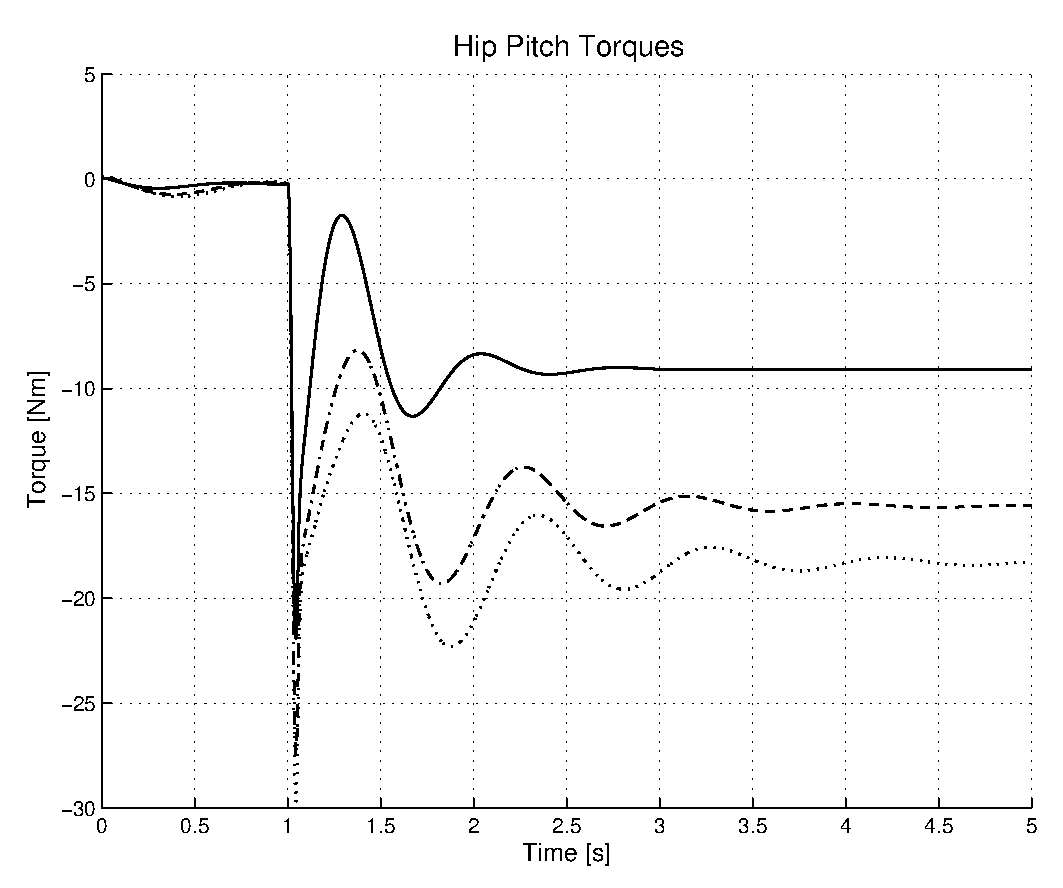
\includegraphics[scale=0.45]{fig/toolchain/casestudy-hip.eps}}
	\subfigure{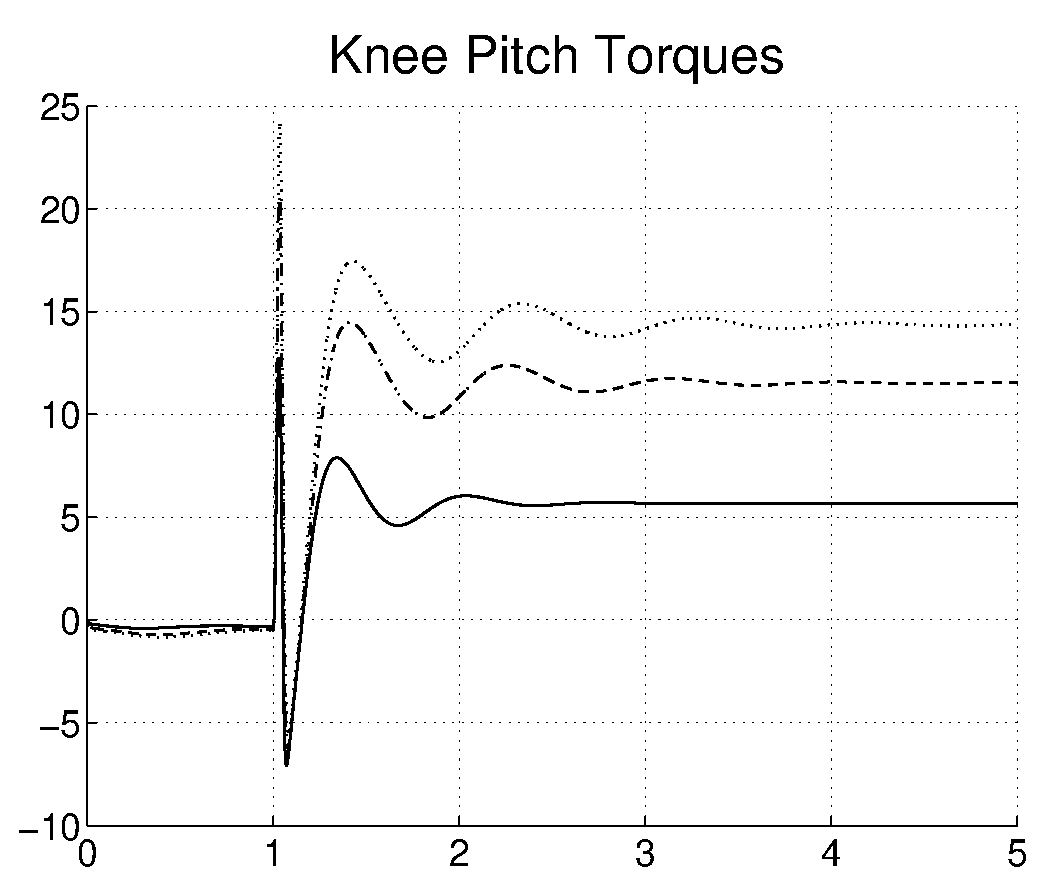
\includegraphics[scale=0.45]{fig/toolchain/casestudy-knee.eps}}
	\end{center}
  	\caption{Hip and knee joint torque requirements while a leg is raised for different sets of motors at the joints.}
	\label{fig:casestudy}
\end{figure}

By using the toolchain, the user can maintain multiple configurations of the same mechanical design in CAD and export them for direct comparison with the dynamic simulator. Since the model is already defined, exporting each configuration takes less than a minute. The parameters of these configuration files can be used along with the model update feature to simulate each configuration and compare the results. In the case of bending the knee and hip joints, there may be several choices of motors which alter the system performance (due to large masses further down the leg). The torque profiles of each joint can be analyzed in the simulation (as shown in Figure \ref{fig:casestudy}) to select the most desirable configuration. The dotted and solid lines represent the heaviest and lightest motors, respectively. The dashed line represents the motor set with medium weight (between the heavy and light motors). The toolchain allows for fast incremental changes to revise the mechanical design and compare the torque requirements. 

% subsection dynamic_simulations (end)

\subsection{Visualization} % (fold)
\label{sub:visualization}
Additional meshes can also be added to the scene to serve as visual aids. For example, coordinate systems can be visualized during simulation by attaching arrow meshes to each link. Alternatively, common Simulink blocks can be used to determine if a particular joint is out of its limits and use the resulting signal to drive the colour of the mesh file (i.e. turn a link \emph{red} if the joint is out of its limits). A particularly useful visual aid for floating base multibody systems is the ability to see where the COM of the system is during simulation.  An additional mesh can be added to the scene driven by the COM calculation from forward kinematics at each time step. The use of this visual aid is shown in Figure  \ref{fig:visualcom}.

\begin{figure}[!h]
	\centering
    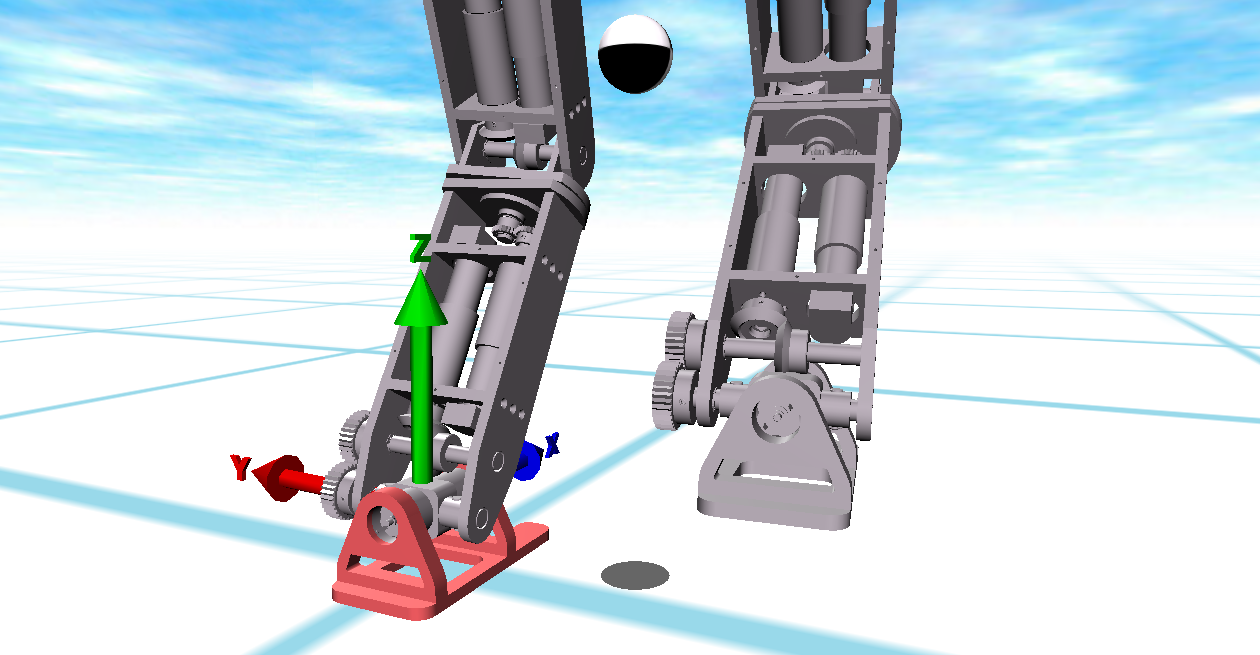
\includegraphics[scale=0.40]{fig/toolchain/visualizecom.png}
  	\caption{Realtime visualization during simulations allows the user to get immediate visual feedback on important information like COM position.}
	\label{fig:visualcom}
\end{figure}

\begin{table}[!h]
  \centering
  \caption{60s Dynamic Simulation Runtime}
    \begin{tabular}{lc}
    \addlinespace
    \toprule
    \textbf{Configuration} & \textbf{Runtime ($s$)}\\
    \midrule
    No Visualization 				& 47.50 	\\
    SimMechanics Visualization    	& 367	 	\\
    Proposed Toolset Visualization 	& 49 		\\
    \bottomrule
    \end{tabular}
  \label{tab:benchmark}
\end{table}

By having the visualization rendered in an external application, the proposed toolchain is capable of running simulations much faster than the built-in 3D viewing capabilities of SimMechanics. This is due to the fact that SimMechanics is unable to parallelize the multibody simulations and visualization. This increase in runtime speed is especially useful during the design phase where rapid iterations are common. The runtime for a 60s dynamic simulation\footnote{The simulations were executed on a standard PC available at the time of writing (2.4GHz Intel Core 2 Duo, 4 GB RAM).} at 1KHz \emph{with} visualization is compared in Table~\ref{tab:benchmark}. If the viewer is also being used to render the 3D mesh for each link through supplied VRML files, it takes much longer. In contrast, the proposed toolchain takes a fraction of the time for the exact same system to be simulated. The simultaneous visualization using the QUARC visualization toolset has little or no impact on the simulation speed. In fact, running the same dynamic simulation without the QUARC visualization toolset only reduces the overall runtime slightly.

% subsection visualization (end)

% section case_study (end)

\section{Summary} % (fold)
\label{sec:toolchain_summary}
A streamlined toolchain was developed to enable rapid prototype development of complex multibody systems. The design process for these systems starts from a mechanical design in CAD, transferring the kinematic/dynamic parameters to a dynamic simulation environment for analysis and revising the design to improve its performance. While a wide range of dynamic simulators already exist, very few of them provide the functionality to directly  import the kinematic/dynamic parameters from CAD. The toolchain provides a semi-automated two-step process for extracting the relevant parameters from CAD and automatically generating the equivalent model in a dynamic simulator. 

The CAD export process is activated through a native plug-in developed for SolidWorks. The plug-in processes each link subassembly file to extract key physical parameters (kinematic/dynamics) and tessellates the surface of each link to generate a 3D mesh for visualization. During the initial export, the user is presented with a simple drag-and-drop interface to specify the kinematic hierarchy of links and joint definitions for the system. The extracted physical and visualization data are stored as XML files in subdirectory for subsequent model generation. 

By storing the extracted data in the universal XML format, routines can be programmed to regenerate the CAD-equivalent model for almost any dynamic simulator. A model generation counterpart was developed for the MATLAB/Simulink environment. Calling a single function in MATLAB automatically parses the exported data and generates full dynamic simulations in Simulink using SimMechanics and 3D visualization using the QUARC toolbox. After the initial model generation, subsequent exports only update the physical model parameters and/or visualization blocks enabling faster design iterations. 

The toolchain was used extensively during the design and development of the 14 DOF biped, demonstrating its usefulness in designing a physical robot. Through the use of visualization aids (i.e. for COM and ZMP position), it was very easy to analyze the behaviour of the initial electromechanical design (from Chapter~\ref{cha:design}) under control action. The forward dynamics and 3D visualization generation proved to be a tremendous benefit during the development of the walking control strategy discussed in the following chapter.
% section discussion (end)

% chapter toolchain (end)

    \chapter{3D Foot Placement Estimator and Gait Generation} % (fold)
\label{cha:simulations}

This chapter extends the Foot Placement Estimator (FPE) algorithm for 3D bipedal robots. Section~\ref{sec:extension_to_3d} presents the method of extending the existing 2D theory (reviewed in Section~\ref{sub:related_foot_placement}) to 3D movement. The proposed algorithm selects a 2D plane in the chosen direction of motion and generates trajectories to produce a forward momentum along the plane. A whole body motion control framework coupled with a finite state machine is used to track the generated trajectories and form complete gait cycles. The toolchain described in the preivous chapter is used to generate dynamic simulations for the 14 DOF bipedal robot and the proposed extension to 3D is validated (Section~\ref{sec:simulations_and_results}).

\section{FPE Extension to 3D} % (fold)
\label{sec:extension_to_3d}

In order to extend the FPE approach to the 3D case, the concept of generating complete gait cycles described in Section~\ref{sub:gait_cycles} is revisted. The primary goal of the first three states in each step cycle (\textbf{PUSH}, \textbf{LIFT} and \textbf{SWING}) is to force the biped into an unstable configuration so that the FPE algorithm can be used to regain stability in the terminal state (\textbf{DROP}).

To extend the 2D algorithm to the general 3D case, we begin by selecting a suitable plane in 3D space as the sagittal plane. The off-sagittal plane is perpendicular to the sagittal plane and the ground.  In the proposed approach, the goal of each step cycle is to control the motion of a 3D bipedal robot to generate a forward moving momentum \emph{along} the selected sagittal plane. Upon entering the terminal state, the FPE equation (\ref{eq:fpe}) is solved on the selected plane to determine the swing foot placement and ultimately regain stability. Unlike the 2D case, consider a 3D bipedal robot with finite foot length and width rather than a biped with point feet as demonstrated in \cite{Wight:2008vt}. The larger size of the region of support increases robustness to these approximation errors. 

The remainder of this thesis assumes a 3D bipedal robot with $n$ actuated degrees of freedom (DOF) and $n+6$ generalized coordinates defined by (\ref{eq:eom1}). 

\subsection{Sagittal Plane} % (fold)
\label{sub:sagittal_plane}
To select an appropriate sagittal plane for a 3D bipedal robot, a vertical plane which lies between the current position of the stance foot and the desired direction of motion is chosen. For a 3D biped walking in a forward motion, this plane is chosen as the the vertical plane passing through the midpoint between the hips and parallel to the direction of forward progress. For side-stepping motion, the coronal plane through the stance foot in the direction of the side step is chosen as the sagittal plane. The selection of the sagittal plane for 3D bipedal robots is illustrated in Figure~\ref{fig:sagittal_plane} for these two situations. 

\begin{figure}[!h]
	\begin{center}
	\subfigure{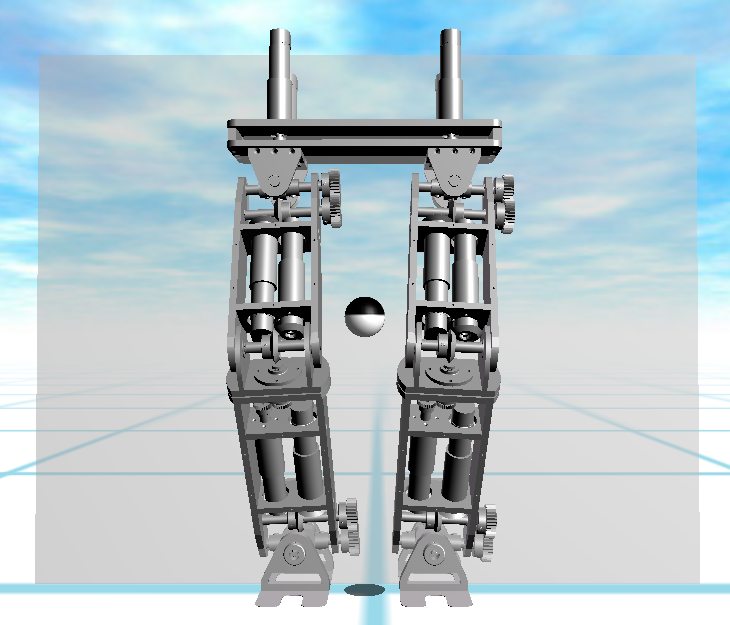
\includegraphics[scale=0.52]{fig/fpe/fpeplanesidestep.png}} 
	\subfigure{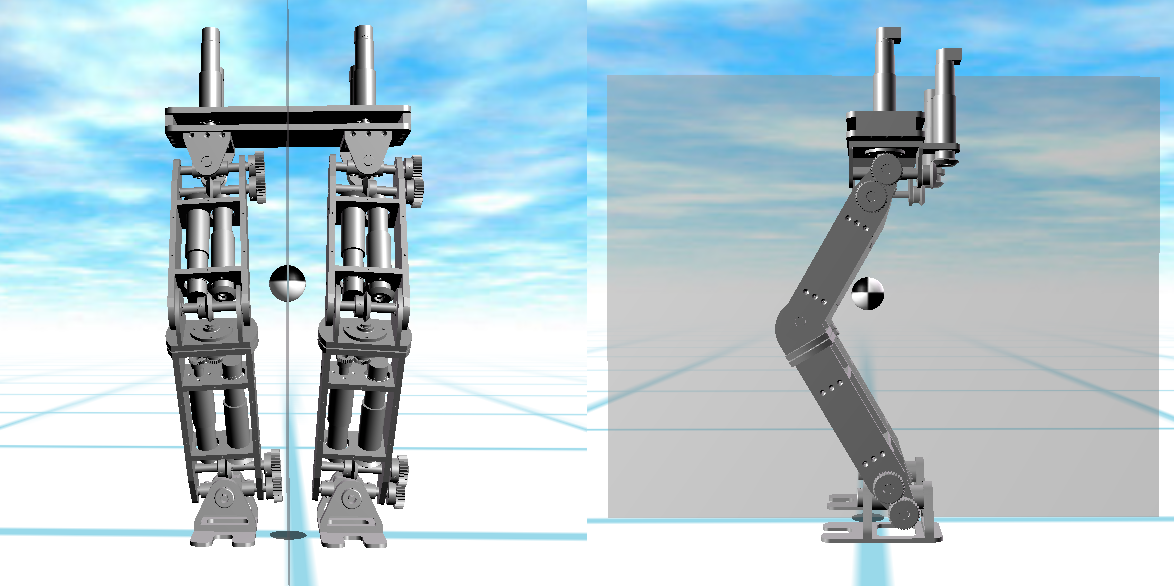
\includegraphics[scale=0.52]{fig/fpe/fpeplaneforwardwalk.png}}
	\end{center}
  	\caption{Sagittal plane selection shown as translucent gray for side-stepping (left) and forward walking (right).}
	\label{fig:sagittal_plane}
\end{figure}

The motion of the biped is controlled based on the selected plane for the duration of the step cycle. During gait initiation, the lines from the COM to the contact points are of length $L$, and the leg separation angle is $\beta$ (similar to the planar case). If the motion of the biped is constrained along this plane, the FPE angle $\phi$ can be used to determine foot placement to regain stability. The parameters required to solve the FPE equation are projected onto the selected plane (additional details are provided in Section~\ref{sub:computing_fpe_parameters}).

Upon impact, the angle $\phi$ converges to $\beta/2$ and a new sagittal plane can be selected for the subsequent step cycle prior to the swing leg entering the \textbf{PUSH} state. Once selected, the stance foot is rotated for alignment and swing leg trajectories can be generated along the plane. By selecting a plane between the current and desired directions of motion, this approach can achieve turning with each step.

% subsection sagittal_plane (end)

\subsection{Trajectory Generation} % (fold)
\label{sub:trajectory_generation}
Once the sagittal plane has been identified at the beginning of each step cycle, appropriate task space trajectories must be generated for the COM ($x_{COM}$) and the swing foot ($x_{SWING}$). In the 2D case, the main goal of the initial states \textbf{PUSH}, \textbf{LIFT} and \textbf{SWING} was to achieve enough forward motion to destabilize the biped. In the 3D case, the robot must also remain stable in the off-sagittal plane while achieving the desired sagittal plane motion. If the ZMP leaves the region of support formed by the stance foot as the swing foot is lifted, the biped begins to fall in the off-sagittal plane and the solution to the 2D FPE equation is insufficient to maintain stable gait. To ensure both forward progress and off-sagittal plane stability, the generated trajectories for $x_{COM}$ are shown in Figure~\ref{fig:comtraj3d}. \\

\begin{figure}[!h]
	\centering
    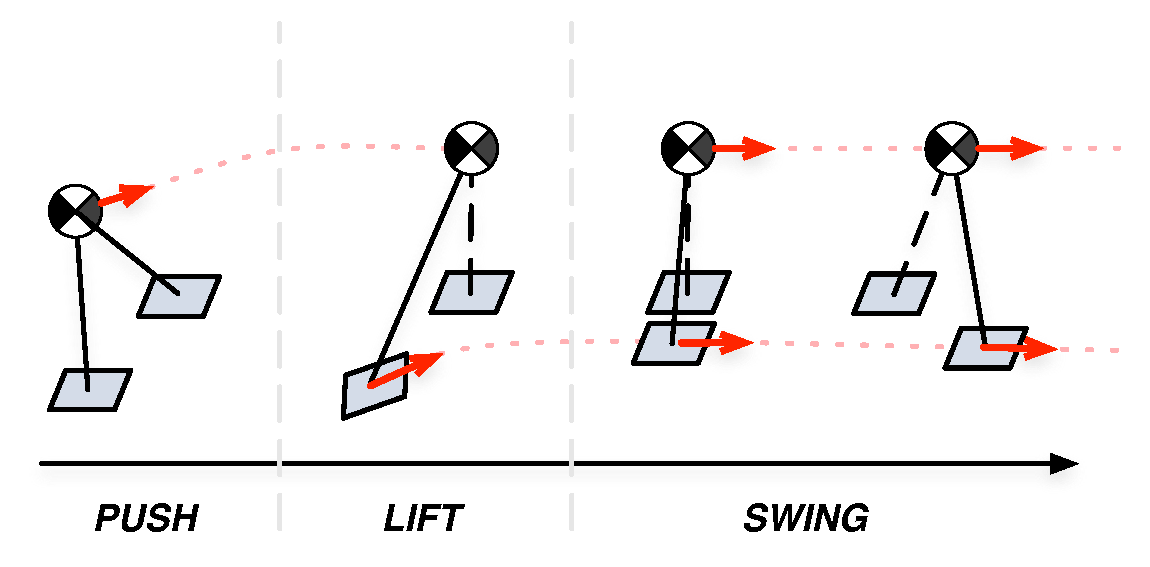
\includegraphics[scale=0.8]{fig/fpe/comtraj3d.eps} 
  	\caption{Trajectory for $x_{COM}$ to ensure forward progress and off-sagittal stability for 3D FPE.}
	\label{fig:comtraj3d}
\end{figure}

\textbf{PUSH}: $x_{COM}$ is moved above the leading stance foot to maintain stability in the off-sagittal and sagittal planes.

\textbf{LIFT}: $x_{COM}$ is held at its current location (above stance foot) while the swing foot is lifted from the ground to achieve sufficient clearance.

\textbf{SWING}: $x_{COM}$ is held in place until the swing foot is aligned with the stance foot in the off-sagittal plane. At this point the $x_{COM}$ is deliberately pushed outside the region of support in the sagittal plane direction. \\

A similar approach is used to generate trajectories for $x_{SWING}$ to achieve the desired behaviour of generating enough momentum to destabilize the biped in the sagittal plane while maintaining stability in the off-sagittal plane. Trajectories for $x_{SWING}$ (illustrated in Figure~\ref{fig:swingfoottraj}) are always computed to align with the sagittal plane formed by the stance foot at the start of the step cycle. This ensures that the solution to the 2D FPE equation remains valid as the \textbf{DROP} state is entered. \\

\textbf{PUSH}: $x_{SWING}$ is held in place as the $x_{COM}$ trajectory is tracked.

\textbf{LIFT}: $x_{SWING}$ follows a ramped trajectory to simultaneously raise the foot off the ground and move it forward in the sagittal plane.

\textbf{SWING}: $x_{SWING}$ follows a straight line trajectory at a specific ground clearance (shown as $h_{LIFT}$ on Figure~\ref{fig:swingfoottraj}) until it reaches the FPE angle $\phi$. \\

\begin{figure}[!h]
	\centering
    \includegraphics[scale=0.8]{fig/fpe/swingfoottraj.eps} 
  	\caption{Trajectory for $x_{SWING}$ along the selected (sagittal) $xz$-plane for 3D FPE.}
	\label{fig:swingfoottraj}
\end{figure}

The ramp trajectory used to raise the swing foot during \textbf{LIFT} should be parameterized in terms of the velocity of the FPE point so that this state transitions faster in the event of larger disturbances (since the biped would have a shorter amount of time to swing the foot over and catch itself).

Depending on the supervisory control mode (i.e. \textbf{WALK} or \textbf{STAND}), the swing leg trajectory can be adjusted to implicitly achieve a desired goal. During \textbf{WALK} mode, the swing foot trajectory tracks a point on the ground slightly behind the FPE point. This under stepping behaviour results in the biped having enough forward moving momentum when the swing foot comes in contact with the ground such that the biped is unstable. As a result, the FPE point is continuously moving forward causing the state machine to transition into the opposing foot's \textbf{LIFT} state upon contact. In the \textbf{STAND} mode, the swing foot trajectory is adjusted to overstep the FPE point so that the biped comes to a stop following this step.

% subsection task_space_trajectory_generation (end)

\subsection{Control Strategy} % (fold)
\label{sub:control_strategy}

A hybrid control strategy is used to simultaneously maintain stability in the off-sagittal plane, achieve sufficient forward momentum along a selected sagittal plane and ultimately track the FPE location to regain stability by taking a step. Similar to the approach presented in \cite{Wight:2008vt}, this approach uses a state machine to transition through the step sequence with each state having a local controller.

During the initial states of the step cycle, whole body motion control is used to track the $x_{COM}$ and $x_{SWING}$ trajectories described in  Section~\ref{sub:trajectory_generation}. To generate the corresponding joint level trajectories, the Jacobian matrix is used to map between the task space and the joint space velocities:

\begin{IEEEeqnarray}{rCl}
	\label{eq:jmap}
	J & = & \begin{bmatrix} \partial q_{act} & \partial x_{base} \\ \end{bmatrix}_{m \times (n+6)}
\end{IEEEeqnarray}

A prioritized task space control scheme is used to generate joint level trajectories which simultaneously achieve state goals while satisfying the highest priority constraint (i.e. holding the $x_{COM}$ position). The state-dependent joint level trajectories can be computed by projecting the lower priority task space goals onto the null space of higher priorities:

\begin{eqnarray}
	\label{eq:priori}
	\dot{q}_{ref} = S(J_{H}^{\#} \dot{x}_{H} + N_{H} J_{L}^{\#} \dot{x}_{L})
\end{eqnarray}

Where, $S = \begin{bmatrix} I_{n \times n} & 0_{n \times 6} \\ \end{bmatrix}$ is the actuator selection matrix for (\ref{eq:gentau}), $J^{\#}$ is the psuedoinverse of the Jacobian $J$, $\dot{q}_{ref}$ is the reference joint velocity, and $\dot{x}_H$ and $dot{x}_L$ are the high and low priority task space velocities, respectively. $J_{H}$ are $J_{L}$ are the corresponding high and low priority Jacobians, and $N_{H} = I - J_{H}^{\#} J_{H}$ is the null space projection matrix. The reference joint velocities are integrated to obtain the reference command signal to be tracked by high gain local Proportional-Derivative (PD) controllers. The specific prioritization of each state is discussed in Section~\ref{sub:joint_level_control}.

When the biped enters the terminal state, the hybrid control strategy switches to directly computing the joint level commands using inverse kinematics. The PD controller gains of the stance foot ankle are set to $K_{P} = K_{D} = 0$ to allow the biped to pivot and fall forward. Simultaneously, the inverse kinematics for the swing leg is solved directly to track the FPE point along the selected sagittal plane.
% subsection control_strategy (end)

\subsection{State Dependent Controllers} % (fold)
\label{sub:joint_level_control}
This section presents the specific controller formulation used during each state of the gait cycle.

\subsubsection{\textbf{STAND}} % (fold)
\label{ssub:stand}
The goal during this state is to maintain the COM position at the geometric centroid of both feet. In order to remain stable under small disturbances, the Jacobian under double support phase is used to compensate for the error $\Delta x_{COM}$ in the X and Y directions.

\begin{IEEEeqnarray}{rClrCl}
	J_{H} & = &
	\begin{bmatrix}
		J_{Stand} \\
		J_{Swing} \\
		J_{COM} \\
	\end{bmatrix}  &
	\dot{x}_{H} & = &
	\begin{bmatrix}
		0 \\
		0 \\
		\dot{x}_{COM} \\
	\end{bmatrix} \nonumber \\
	J_{L} & = &
	\begin{bmatrix}
		0 \\
	\end{bmatrix}  &
	\dot{x}_{L} & = &
	\begin{bmatrix}
		0 \\
	\end{bmatrix} \nonumber \\
\end{IEEEeqnarray}

% subsubsection stand (end)

\subsubsection{\textbf{PUSH}} % (fold)
\label{ssub:push}
The goal during this state is to track the trajectory generated for $x_{COM}$ to move to the stance foot support region while remaining in the double support phase. An augmented Jacobian matrix is used to track the trajectory while simultaneously maintaining the foothold constraints.

\begin{IEEEeqnarray}{rClrCl}
	J_{H} & = &
	\begin{bmatrix}
		J_{Stand} \\
		J_{Swing} \\
		J_{COM} \\
	\end{bmatrix}  &
	\dot{x}_{H} & = &
	\begin{bmatrix}
		0 \\
		0 \\
		\dot{x}_{COM} \\
	\end{bmatrix} \nonumber \\
	J_{L} & = &
	\begin{bmatrix}
		0 \\
	\end{bmatrix}  &
	\dot{x}_{L} & = &
	\begin{bmatrix}
		0 \\
	\end{bmatrix} \nonumber \\
\end{IEEEeqnarray}

The joint level reference velocities are calculated from (\ref{eq:priori}) and integrated to obtain the position command.

% subsubsection push (end)

\subsubsection{\textbf{LIFT}} % (fold)
\label{ssub:lift}
In the lift stage, the highest priority task is maintaining the foothold of the stance foot, holding the $x_{COM}$ directly above it and simultaneously raising the swing foot from the ground. The key challenge in this state is that lifting the swing foot can potentially cause the centre of pressure to leave the support region formed by the contact points of the stance foot. The prioritized task space control scheme is used to generate joint level commands to track the $x_{SWING}$ trajectory while satisfying the higher priority goal of maintaining the foothold and balance.

\begin{IEEEeqnarray}{rClrCl}
	J_{H} & = &
	\begin{bmatrix}
		J_{Stance} \\
		J_{COM} \\
	\end{bmatrix} &
	\dot{x}_{H} & = &
	\begin{bmatrix}
		0 \\
		\dot{x}_{COM} \\
	\end{bmatrix} \nonumber \\
	J_{L} & = &
	\begin{bmatrix}
		J_{Swing} \\
	\end{bmatrix}  &
	\dot{x}_{L} & = &
	\begin{bmatrix}
		\dot{x}_{Swing} \\
	\end{bmatrix} \nonumber \\
\end{IEEEeqnarray}

The joint level reference velocities are calculated from (\ref{eq:priori}) and integrated to obtain the position command.

% subsubsection lift (end)

\subsubsection{\textbf{SWING}} % (fold)
\label{ssub:swing}


At this point, the goal of the control approach is to generate a forward moving momentum along the selected sagittal plane. This deliberately destabilizes the biped by pushing $x_{COM}$ outside the region of support in the chosen direction of motion. The task space prioritization in this state remains consistent with the previous state until the biped is unstable, at which point the control strategy enters the terminal \textbf{DROP} state.

\begin{IEEEeqnarray}{rClrCl}
	J_{H} & = &
	\begin{bmatrix}
		J_{Stance} \\
		J_{Swing} \\
	\end{bmatrix} &
	\dot{x}_{H} & = &
	\begin{bmatrix}
		0 \\
		\dot{x}_{Swing} \\
	\end{bmatrix} \nonumber \\
	J_{L} & = &
	\begin{bmatrix}
		J_{COM} \\
	\end{bmatrix}  &
	\dot{x}_{L} & = &
	\begin{bmatrix}
		\dot{x}_{COM} \\
	\end{bmatrix} \nonumber \\
\end{IEEEeqnarray}

The joint level reference velocities are calculated from (\ref{eq:priori}) and integrated to obtain the position command.
% subsubsection swing (end)

\subsubsection{\textbf{DROP}} % (fold)
\label{ssub:drop}
In this terminal state, the Jacobian is used to track the fixed stance foot position and the generated swing foot trajectory to track the FPE point on the ground. Since the ZMP is outside of the region of foot support during this state, the torso is treated as a fixed base link and compute the Jacobian matrix of each foot.

\begin{IEEEeqnarray}{rClrCl}
	J_{H} & = &
	\begin{bmatrix}
		J_{Stance} \\
		J_{Swing} \\
	\end{bmatrix} &
	\dot{x}_{H} & = &
	\begin{bmatrix}
		\dot{x}_{Stand} \\
		\dot{x}_{Swing} \\
	\end{bmatrix} \nonumber \\
	J_{L} & = &
	\begin{bmatrix}
		0 \\
	\end{bmatrix}  &
	\dot{x}_{L} & = &
	\begin{bmatrix}
		0 \\
	\end{bmatrix} \nonumber \\
\end{IEEEeqnarray}

\subsubsection{\textbf{CONTACT STABILIZATION}} 

With an arbitrary 3D biped with finite sized feet, it is possible for the biped to land on the edge of the foot instead of landing perfectly above the FPE point on the ground. Once ground contact is made, the solution to the FPE equation is no longer valid (since a real biped will not have instantaneous transfer of balance). To handle this behaviour, a stabilization substate is used where the joint level control is computed directly. At this point, trajectories are generated for the ankles to align the surface of the foot with the ground and switch to high gain PD control for tracking. This ensures that both feet are in full contact with the ground prior to executing the opposite leg's gait sequence. The biped-ground contact interface is shown before and after the stabilization substate in Figure~\ref{fig:contact_stabilization}. 

\begin{figure}[!h]
	\begin{center}
	\subfigure{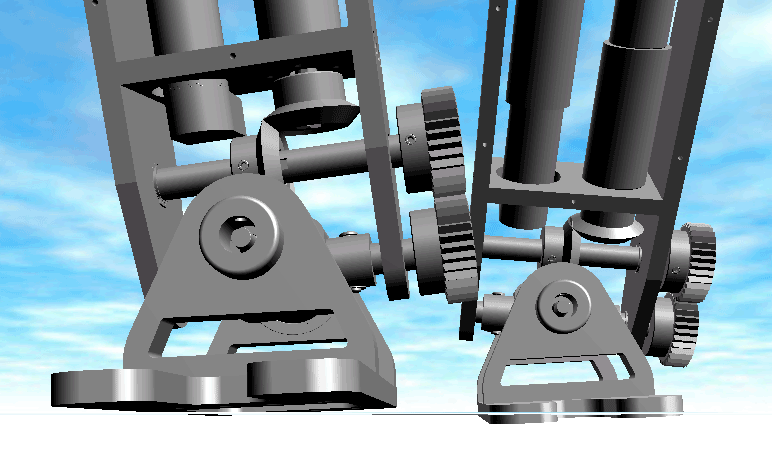
\includegraphics[scale=0.29]{fig/fpe/prestabilization.png}} 
	\subfigure{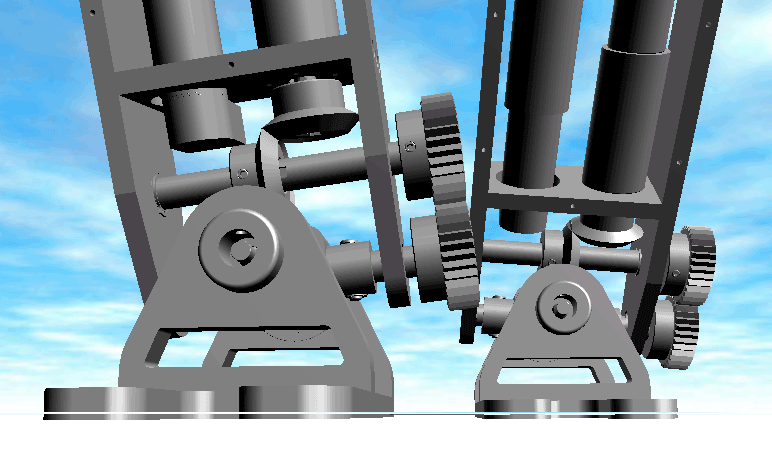
\includegraphics[scale=0.29]{fig/fpe/poststabilization.png}}
	\end{center}
  	\caption{Ground-foot contact shown for before (left) and after (right) contact stabilization.}
	\label{fig:contact_stabilization}
\end{figure}


% subsubsection drop (end)

% subsection joint_level_control (end)

\subsection{Computing the FPE Parameters} % (fold)
\label{sub:computing_fpe_parameters}
The 2D FPE equation (\ref{eq:fpe}) requires the total inertia about the COM ($I_{COM}$) and average angular velocity about the pivoted fixed foot ($\dot{\theta}_{avg}$). In the 2D case, the moment of inertia for link $k$ is a scalar value since there is only one plane of rotation. The total inertia about the COM is computed by summing the moment of inertia for each link in the system. In the 3D case, the moment of inertia for each link is a $3\times3$ tensor: 

\begin{equation}
	\begin{aligned}
		{I_k} = \left[ {\begin{array}{*{20}{c}}
{{I_{xx}}}&{{I_{xy}}}&{{I_{xz}}}\\
{{I_{yx}}}&{{I_{yy}}}&{{I_{yz}}}\\
{{I_{zx}}}&{{I_{zy}}}&{{I_{zz}}}
\end{array}} \right]
	\end{aligned}
\end{equation}

The inertia tensor of each link is taken at the COM aligned with the local coordinate system. If the $xz$-plane is selected as the sagittal plane in 3D space, the moment of inertia of link $k$ is the $I_{yy}$ term. However, in the 3D case the motion of the biped is no longer fixed to a single plane of rotation. By attaching a fixed coordinate frame to the selected sagittal plane at the start of each step, the orientation of the sagittal plane can be expressed as a $3\times3$ rotation matrix $R$. The local inertia tensor can be rotated into the selected sagittal plane's coordinate frame by: 

\begin{equation}
	\begin{aligned}
		{I_{k,sagittal}} = R \cdot {I_k} \cdot {R^T}
	\end{aligned}
	\label{eq:isagittal}
\end{equation}

Then the effective moment of inertia of each link \emph{projected on to the selected sagittal plane} can be obtained by transforming the inertia tensor with (\ref{eq:isagittal}) and pulling out the $I_{yy}$ term, $I_{k,yy}$. The total inertia about the COM can then be computed by summing the effective inertia of each link on the sagittal plane: 

\begin{equation}
	\begin{aligned}
		{I_{COM}} = \sum\limits_{k = 1}^n {{I_{k,yy}}}
	\end{aligned}
	\label{eq:icom_3d}
\end{equation}

The average angular velocity is computed as a weighted sum of the inertia of each link \cite{Wight:2008ii}. In the 3D case, the same equation is used with the \emph{effective} moment of inertia of each link on the sagittal plane: 

\begin{equation}
	\begin{aligned}
		{\dot \theta _{avg}} = \frac{{\sum\limits_{k = 1}^n {{I_{k,yy}}} {{\dot \theta }_k}}}{{\sum\limits_{k = 1}^n {{I_{k,yy}}} }}
	\end{aligned}
	\label{eq:wavg_3d}
\end{equation}

The angular velocity of each link ${\dot{\theta}_k}$ is obtained by rotating the joint velocity (expressed as a $3\times1$ vector with $\dot{q}_k$ in the row represented by its local axis of rotation) to the fixed frame of the sagittal plane. 

The parameters computed with (\ref{eq:icom_3d}) and (\ref{eq:wavg_3d}) are plugged in to the 2D FPE equation (\ref{eq:fpe}) and the solution ($\phi$) is obtained with a non-linear equation solver. 
% subsection computing_fpe_parameters (end)

% section extension_to_3d (end)

\section{Simulations and Results} % (fold)
\label{sec:simulations_and_results}

The proposed control strategy to extend the FPE theory to 3D was implemented in simulation on a 14 DOF lower body bipedal robot. Each state of the control strategy was implemented in the Matlab/Simulink environment with the multibody dynamics simulation by SimMechanics. Accurate kinematic and dynamic properties of the physical robot were taken directly from the CAD model through the toolchain model generation process (as discussed in Section~\ref{sec:model_generation}). The controller diagram shown in Figure~\ref{fig:fpecontroller} implements the control strategy presented in this section. The subsystems from the outer most loop working inwards are described as follows: 

\begin{figure*}[!b]
	%\centering
    \centerline{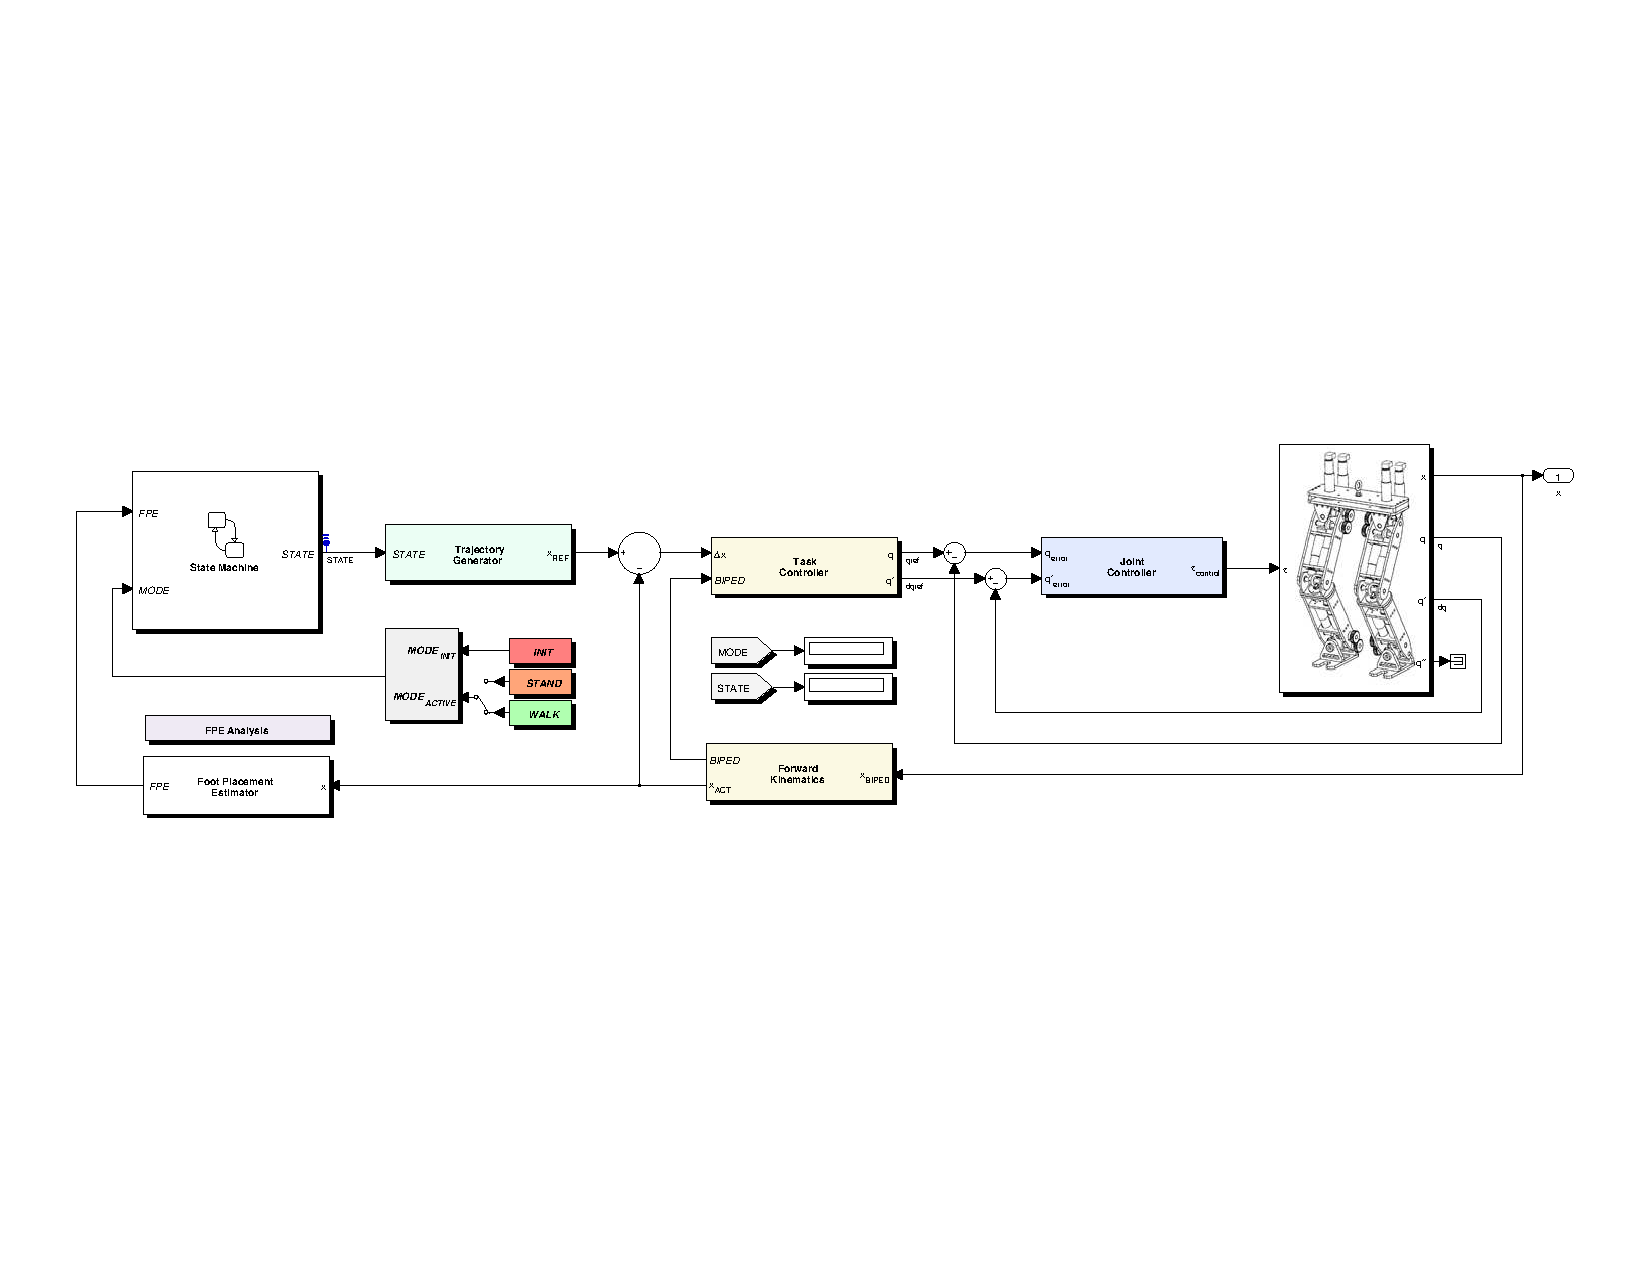
\includegraphics[trim = 12mm 75mm 12mm 75mm,clip,width=18cm]{fig/simulations/fpecontroller.pdf}}
  	\caption{Controller diagram of 3D FPE based walking control strategy implemented in Simulink.}
	\label{fig:fpecontroller}
\end{figure*}

\begin{enumerate}
	\item \textbf{State Machine} \\ 
	Finite state machine logic was implemented in Stateflow as shown in Figure~\ref{fig:stateflow}. The state names follow the same convention as the 2D FPE case (shown in Figure~\ref{fig:statemachine}) while the transition logic is updated for the 3D case described in Section~\ref{sub:joint_level_control}.  \\

	\item \textbf{Trajectory Generator} \\ 
	Generates the task space COM ($x_{COM}$) and the swing foot ($x_{SWING}$) trajectories detailed in Section~\ref{sub:trajectory_generation} based on the current state of the controller. Also uses the higher level supervisory control mode (i.e. \textbf{WALK} or \textbf{STAND}) to adjust the trajectory generation for understepping/overstepping the FPE point. \\

	\item \textbf{Foot Placement Estimator} \\ 
	Computes the FPE parameters about the COM ($I_{COM}$, $\dot{\theta}_{avg}$) for the 3D case (detailed in Section~\ref{sub:computing_fpe_parameters}) and solves the FPE equation (\ref{eq:fpe}) using a numerical methods-based nonlinear solver from \cite{Wight:2008vt}. \\

	\item \textbf{Task Controller} \\ 
	Provides the state dependent control logic for the whole body motion control framework in Section~\ref{sub:control_strategy}. The resulting joint space velocities are integrated to obtain the joint position reference command. The contact stabilization substate used in the second half of \textbf{DROP} is also implemented here to generate joint level trajectories directly. \\

	\item \textbf{Joint Controller} \\ 
	High gain joint level PD controllers with gain scheduling based on the current state of the control strategy. The output of this block ($\vtau$) is used to drive the forward dynamics simulation generated with the toolchain. \\

\end{enumerate}

\begin{figure}[!h]
	\centering
    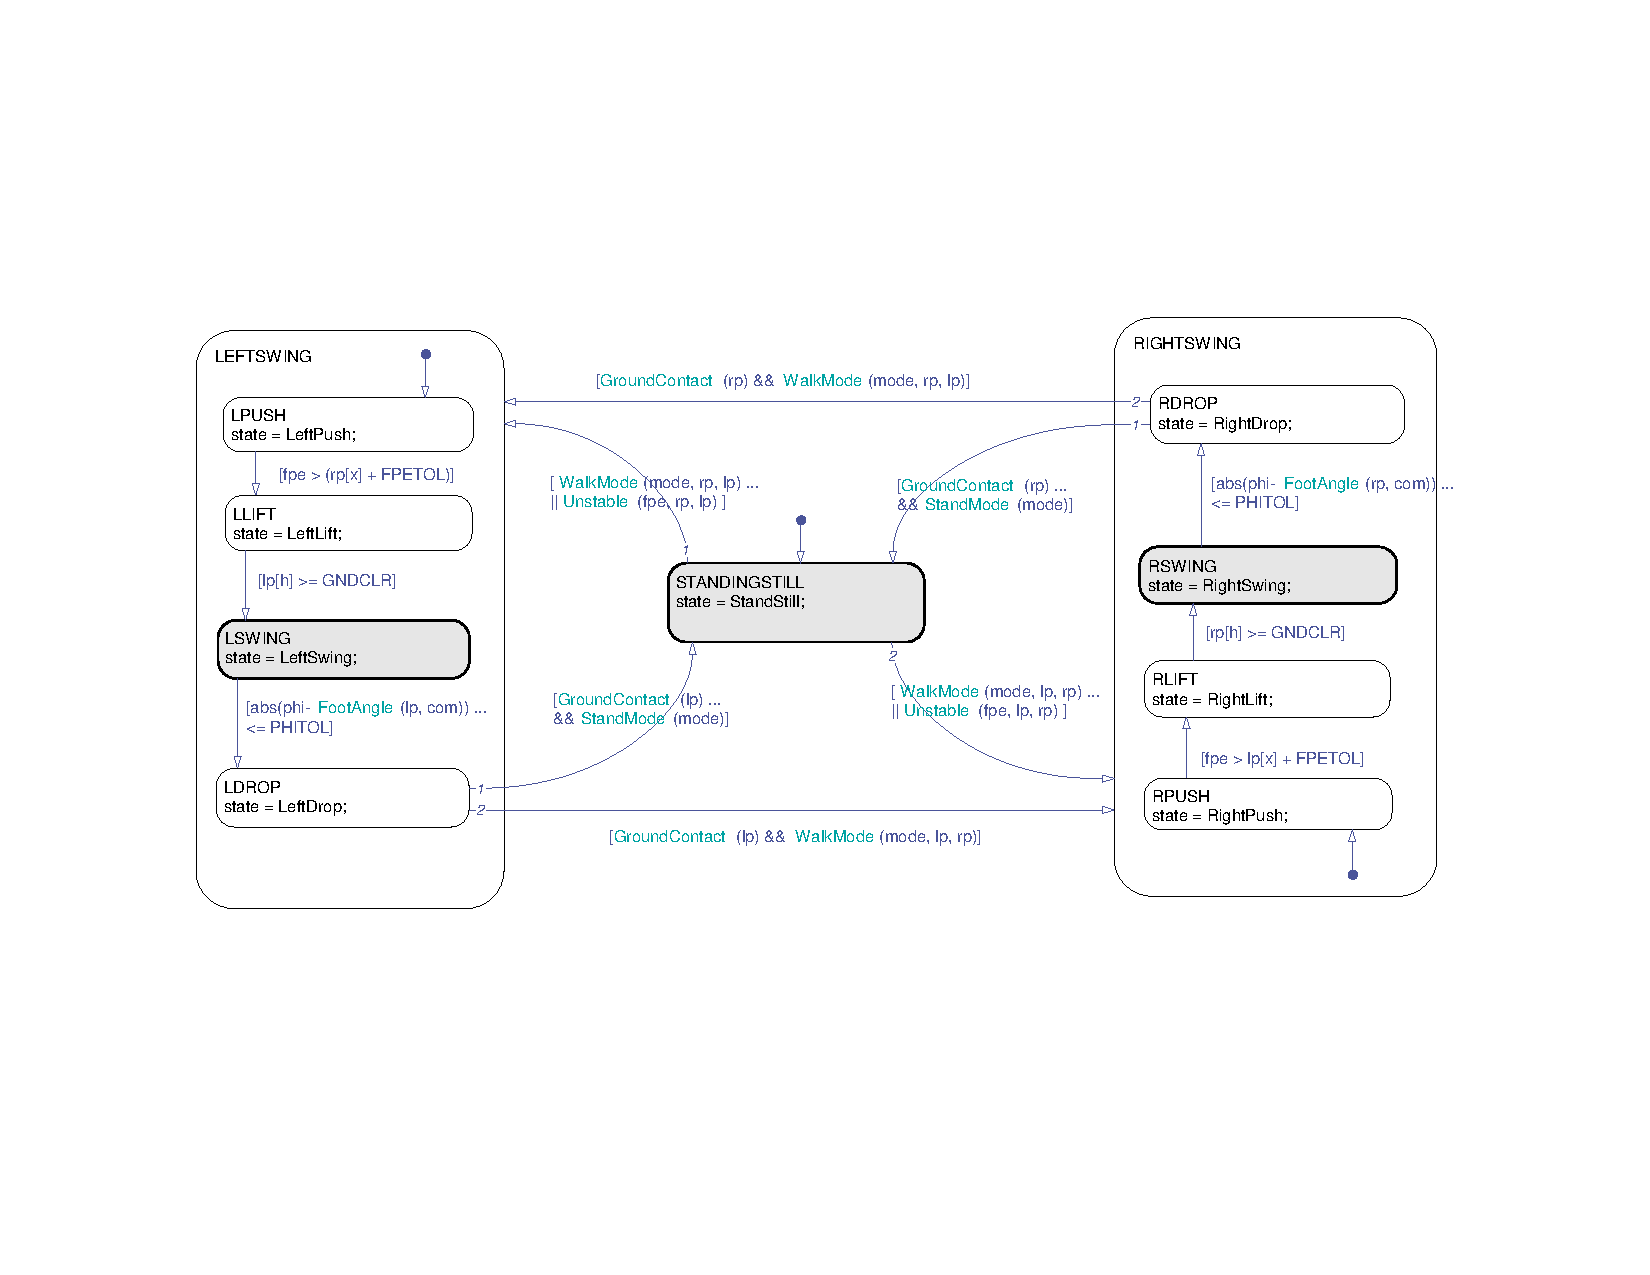
\includegraphics[trim = 30mm 60mm 25mm 53mm,clip,width=17cm]{fig/simulations/statemachine.pdf} 
  	\caption{Finite state machine implemented in Stateflow for 3D FPE-based walking control strategy.}
	\label{fig:stateflow}
\end{figure}

The simulations are executed with a fixed step Runge-Kutta solver at 1KHz. The forward dynamics generated with the toolchain drive the simultaneous 3D visualizations in an external viewer application.  

\subsection{Contact Modeling} % (fold)
\label{sub:full_contact_modeling}
The initial spring-damper contact model discussed in Section~\ref{sub:initial_contact_modeling} was replaced with a more complex version to accurately model the ground/foot dynamics. The Hunt and Crossley contact model \cite{hunt1975coefficient,gilardi2002literature} generates a normal force using a non-linear spring-damper system defined by: 

\begin{equation}
	\label{eq:contacthc}
	{F_{normal}} = b{z^p}{\dot z^q} + k{z^n}
\end{equation}

Where $z$, $\dot{z}$ are the penetration depth position and velocity, respectively. The constants $k$, $b$ are the spring-damper coefficients and $n$, $p$, $q$ are tunable constants. Equation (\ref{eq:contacthc}) provides the ground reaction force in the normal direction only. The tangential (frictional) contact forces were modeled by: 


\begin{equation}
	\label{eq:contactfr}
	{F_{tangential}} = f{\dot x}
\end{equation}

Where $\dot x$ is the tangential velocity of the contact point (in the $x$ and $y$ directions) and $f$ is a tunable constant. The forces generated by (\ref{eq:contacthc}) and (\ref{eq:contactfr}) ensure that there are no discontinuities when ground contact is made. A seperate dynamic simulation model was generated to tune the contact model constants to emulate a stiff ground. The final (tuned) parameters used for dynamic simulations are provided in Table~\ref{tab:contactk}.

\begin{table}[!h]
  \centering
  \caption{Tuned contact model constants.}
    \begin{tabular}{cc}
    \addlinespace
    \toprule
    \textbf{Parameter} & \textbf{Value}\\
    \midrule
	$f$	&	10 \\
    $k$	&	2000 \\
    $b$	&	10 \\
    $p$	&	1.10 \\
    $q$  &	1.00 \\
    $n$	&	2.31 \\
    \bottomrule
    \end{tabular}
  \label{tab:contactk}
\end{table}

It was found that stiffening the ground contact by raising the model constants would produce singularities with fixed time step simulations at 1 KHz. Reducing the time step helped avoid singularities but the simulation runtime drastically increased. 
% subsection contact_modeling (end)

\subsection{Side-to-Side Stepping} % (fold)
\label{sub:3d_simulations}

\begin{figure}[!h]
	\centering
    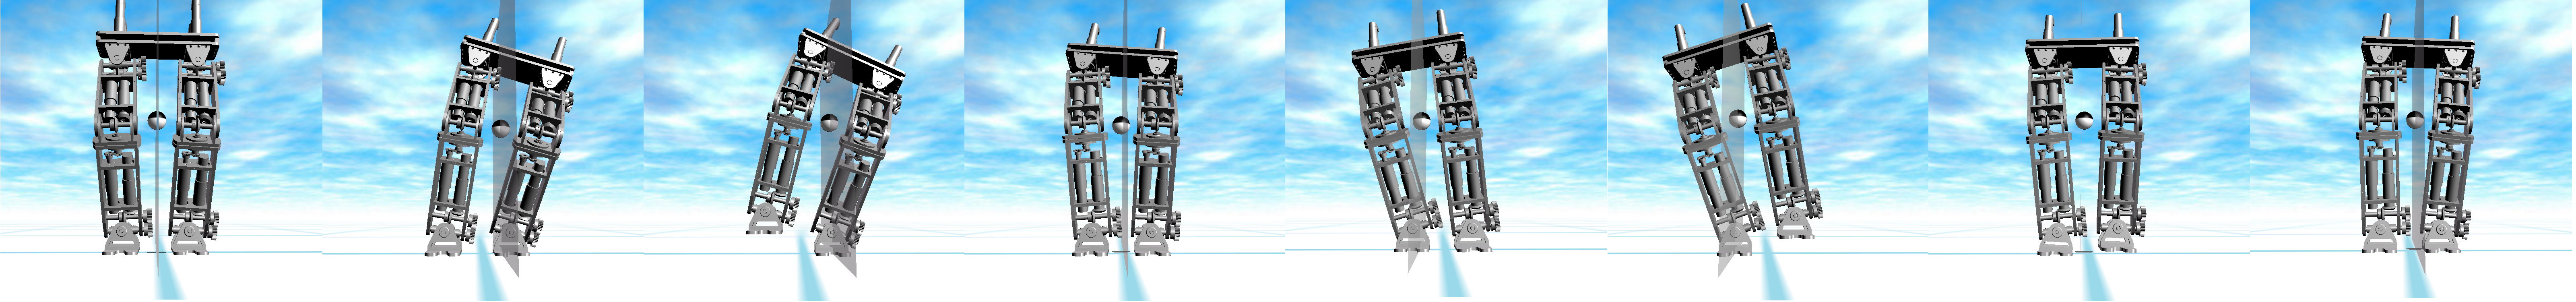
\includegraphics[scale=0.095]{fig/simulations/sidesequence.png}
  	\caption{Frame captures from the realtime 3D visualization while side-to-side stepping.}
	\label{fig:sidesequence}
\end{figure}

To demonstrate the dynamic stability of a 3D biped under this approach, the frontal plane was selected as the sagittal plane. Forward motion along this sagittal plane results in a side-to-side stepping sequence for the biped (as shown in Figure \ref{fig:sidesequence}). The gray plane in the frame captures moves along the Y-direction (biped's frontal plane). The intersection of the gray plane and the ground indicates the FPE point tracked during \textbf{DROP}. 

The resulting $x_{COM}$ trajectories from simulating the side-to-side stepping motion (shown in Figure \ref{fig:sidecomtraj}) demonstrate the stability of the biped through a complete gait sequence. The prioritized motion control framework handles the dynamic switching of constraints (from double support to single support) while generating the appropriate joint level commands for swinging the COM over. The colour coded dotted lines on Figure \ref{fig:sidecomtraj} indicate the boundaries of each foot on the ground. Note that during the \textbf{SWING} state, the COM is pushed outside the region of support (around 11s). This in turn initiates the \textbf{DROP} state where the FPE point is tracked to regain stability.

\begin{figure}[!h]
	\centering
    \includegraphics[scale=0.6]{fig/simulations/sidecomtraj.eps}
  	\caption{COM trajectory being tracked during the complete gait sequence of side stepping.}
	\label{fig:sidecomtraj}
\end{figure}


In the terminal \textbf{DROP} state, the swing foot trajectory tracks the FPE point on the ground (shown in Figure \ref{fig:sidefpetrack}) with an added offset to ensure that the biped oversteps to guarantee stability (as per the 2D FPE theory). Once ground contact is made (around 11.6s), the stabilization substate is entered and the swing foot trajectory is controlled directly to align the foot with the ground. This causes the biped to rock back and forth (similar to the 2D case) until stability is reached.

\begin{figure}[!h]
	\centering
    \includegraphics[scale=0.6]{fig/simulations/sidefpetrack.eps}
  	\caption{Swing foot tracks the a point on the ground given by $FPE + FPE_{offset}$ to ensure overstepping.}
	\label{fig:sidefpetrack}
\end{figure}


\subsection{Forward Walking Gait} % (fold)
\label{sub:forward_walking_gait}
\Incomplete 

\begin{figure}[!h]
	\centering
    \includegraphics[scale=0.6]{fig/simulations/fwdcomtraj.eps}
  	\caption{COM and foot trajectories in the direction of forward progress and off-sagittal plane during a complete gait cycle.}
	\label{fig:fwdcomtraj}
\end{figure}

\begin{figure}[!h]
	\centering
    \includegraphics[scale=0.7]{fig/simulations/fwdfpetraj.eps}
  	\caption{FPE and foot trajectories in the direction of forward progress during a complete gait cycle.}
	\label{fig:fwdfpetraj}
\end{figure}

\begin{figure}[!h]
	\begin{center}
	\subfigure{\includegraphics[scale=0.45]{fig/simulations/fwdlfoottraj.eps}}
	\subfigure{\includegraphics[scale=0.45]{fig/simulations/fwdrfoottraj.eps}}
	\end{center}
  	\caption{Foot trajectories on the selected sagittal plane during a complete gait cycle.}
	\label{fig:fwdfoottraj}
\end{figure}

% subsection forward_walking_gait (end)

% section simulations_and_results (end)

\section{Summary} % (fold)
\label{sec:simulations_summary}
The FPE theory is extended to the 3D case to form dynamically stable gait cycles by selecting a 2D sagittal plane parallel to the desired direction of motion. The primary goal in the 3D case is to generate a forward momentum along this selected sagittal plane. For the duration of the step cycle, the FPE equation is used to determine the appropriate swing foot placement to restore balance from the momentum generated along the plane. A new sagittal plane is selected with each step to enable turning. 

Trajectories are generated for the swing foot and COM position to simultaneously generate the forward momentum along the plane while remaining stable in the off sagittal plane until the \textbf{DROP} state is reached. Upon entering this terminal state, the 3D biped is falling forward in the desired direction of motion and the swing foot tracks the FPE point to restore balance. 

A whole body motion control framework is used to generate the appropriate joint level trajectories during each state of the proposed control strategy. The framework uses a prioritized control scheme where the low priority constraints of each state are projected into the null space of higher priority tasks. This approach handles the dynamic switching of constraints as the biped moves between the single and double support phases. 

The 14 DOF bipedal robot developed in previous chapters is used to demonstrate the control strategy presented in this chapter. Dynamic simulations with 3D visualization are generated directly from the CAD model using the toolchain. The simulations are used to verify the efficacy of the proposed control strategy for side-stepping and forward walking gait. Despite using a more complex contact model, tuning the parameters to accurately model a stiff ground in reality proved to be challenging. This imperfection in the simulation environment highlights the need to develop physical hardware to validate walking control strategies, as presented in the following chapter.
% section discussion (end)

% chapter simulations (end)
    \chapter{Experimental Results} % (fold)
\label{cha:experiments}

This chapter presents the experimental work completed to validate the actuator dynamics and motion control framework. It is important to test walking control strategies on physical hardware directly due to the imperfections in a simulation environment. For example, the contact models used to estimate the ground reaction force is only an approximation. There are also other unmodeled effects which can significantly alter the dynamics of the physical system (i.e. vibrations). The simulations used to demonstrate the proposed 3D FPE walking control strategy in the previous section accounted for link side dynamics only. Section~\ref{sec:actuator_model} describes the modifications to account for the actuator dynamics. This modification to the simulations enables a single controller designed in Simulink to target either the simulation environment or the physical hardware using the HIL architecture discussed in Section~\ref{sec:hil_architecture}. The experimental validation for a single actuator and the proposed motion control framework are presented in Sections \ref{sec:1dof_validation} and \ref{sec:motion_control_validation}, respectively. 

\section{Physical Hardware} % (fold)
\label{sec:physical_hardware}
The electromechanical design presented in Chapter~\ref{cha:design} was realized to develop the 14 DOF bipedal robot (single leg shown in Figure~\ref{fig:bipedleg}). The mechanical implementation was derived directly from the revised CAD models. The electronics used for control hardware were developed by an industry collaboration partner, Quanser Consulting Inc. This section presents the realization of the physical hardware used for experimental validation. 

\begin{figure}[!h]
	\centering
    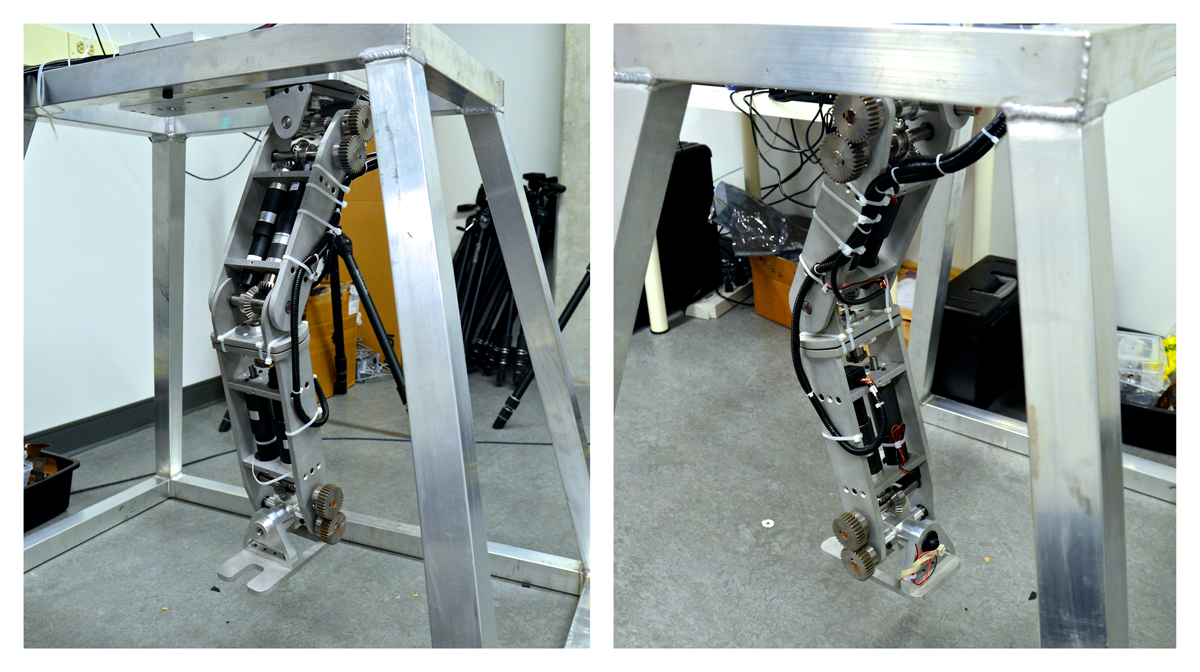
\includegraphics[scale=0.39]{fig/hardware/bipedleg.png} 
  	\caption{The 7 DOF leg built for the bipedal robot based on the electromechanical design in Chapter~\ref{cha:design}.}
	\label{fig:bipedleg}
\end{figure}

\subsubsection{Mechanical Implementation} % (fold)
\label{ssub:mechanical_implementation}

The final mechanical design was developed on campus at the University of Waterloo. The on-site engineering machine shop developed the mechanical chassis components from the final CAD drawings (shown in Appendix~\ref{app:bipedcad}). The selected DC motors and gearhead combinations were sourced from a motor manufacturer. The drivetrain components (i.e. bearings, shafts, gears) used to relocate the output gearhead shaft from each joint axis were also sourced from a hardware vendor. The complete mechanical assembly was completed by the author of this thesis. The completely assembled joints and links of the bipedal robot leg is shown in more detail in Figure~\ref{fig:bipedcloseup}.

\begin{figure}[!h]
	\centering
    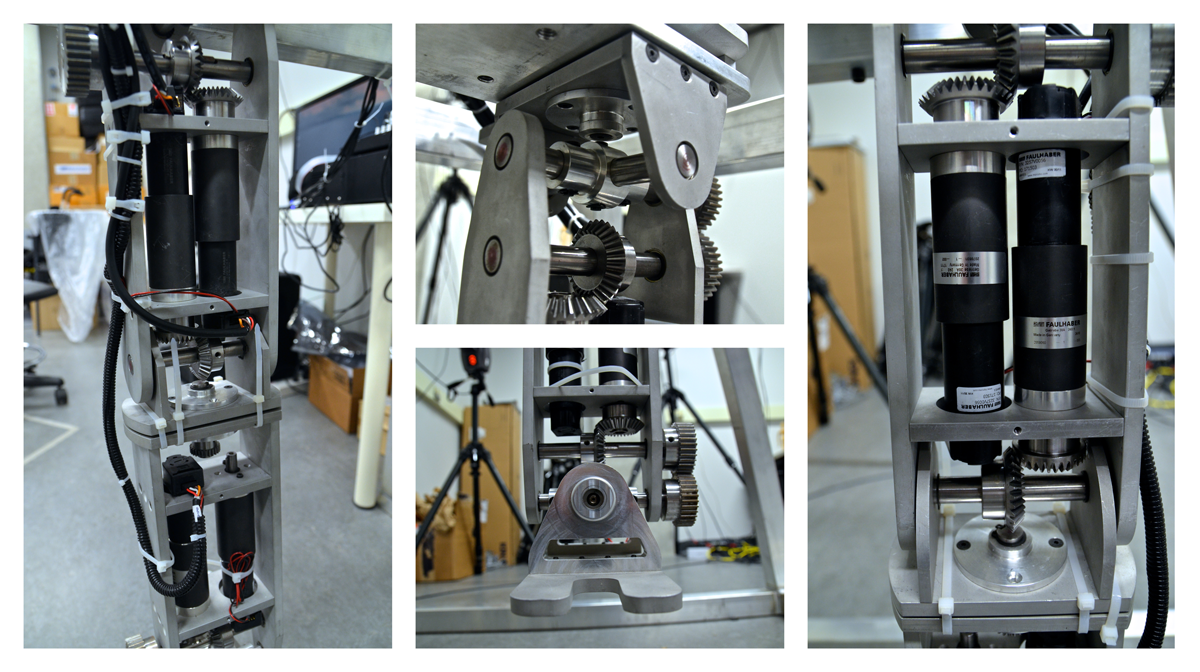
\includegraphics[scale=0.38]{fig/hardware/bipedcloseup.png} 
  	\caption{Close up pictures of various joints and linkages in mechanical implementation of the bipedal robot design.}
	\label{fig:bipedcloseup}
\end{figure}

The mechanical chassis was composed primarily out of Aluminum 5052 and created using Computer Numerical-Controlled (CNC) machine tools directly from the CAD files. This enabled repeatable and accurate positioning of mechanical features in the chassis components (i.e. for the separation of holes for gearing components to mesh well). The use of CNC machine tools was also useful since some chassis components (i.e. motor mounts) were used multiple times in the design of each leg. The advantage here was once the machine was setup to produce the first component, the remaining copies could be produced faster using the same setup. 

One of the key challenges in the assembled leg was the use of bevel gears for perpendicular mechanical coupling. It was difficult to position the gear axis with enough accuracy to achieve perfect clearance between mating components. As a result, some of the joints which use this design approach to shift the weight distribution suffer from backlash (or ``joint play''). In the current design, this is particularly evident for the knee joint, where one of the stock gearing components were modified due to fitment issues. 

In addition to developing the bipedal robot, a supporting frame was also designed for fixed base and (tethered) walking experiments (CAD drawings available in Appendix~\ref{app:framecad}). 
% subsubsection mechanical_implementation (end)

\subsubsection{Control Implementation} % (fold)
\label{ssub:electronics_implementation}

The electronics used for controlling the bipedal robot was developed by an industry collaboration partner. Quanser Consulting Inc developed custom motor controllers and drivers as per the current requirements derived from torque estimates in dynamic simulations. Each joint in the bipedal robot has a (dedicated) local motor controller and driver unit. A control system model developed in Matlab/Simulink using Quanser's QUARC toolbox communicates with the electronics hardware through a serial interface (USB). Quanser's complete system enables hardware-in-the-loop (HIL) experiments with the physical bipedal robot (described further in Section~\ref{sec:hil_architecture}).    

\begin{figure}[!h]
	\centering
    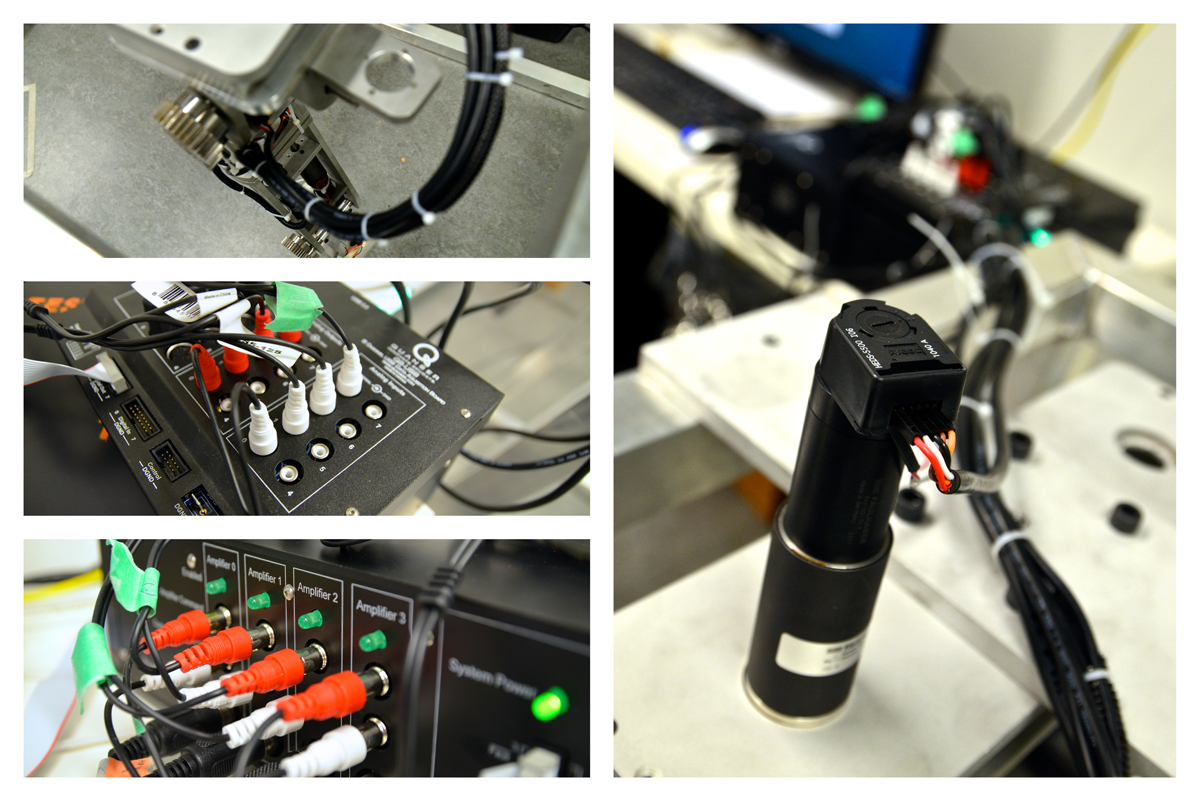
\includegraphics[scale=0.39]{fig/hardware/bipedwired.png} 
  	\caption{Electronics and wiring used to interface control loops running in Simulink to the physical hardware.}
	\label{fig:bipedwired}
\end{figure}

Unfortunately, the electronics hardware developed by Quanser was not ready in time for experimental validation. Since it is a custom solution, further development was required before it could be used to control the complete 14 DOF bipedal robot. Quanser provided the author with control electronics from their existing product offerings in the interim to complete \emph{some} experimental validation on the physical robot. The general idea is that the HIL experiment models developed to target the interim solution could easily be switched to target the custom solution once it is ready for us. The interim solution is hardware constrained to 7 channels available for control and current output per channel. A single 7 DOF leg shown in Figure~\ref{fig:bipedwired} was wired to these channels for \emph{some} experimental validation. 

% subsubsection electronics_implementation (end)

% section physical_hardware (end)

\section{Actuator Model} % (fold)
\label{sec:actuator_model}
PD control is applied for each joint in order to track the desired trajectory generated by higher levels of control (Section~\ref{sub:control_strategy}). The control signal $u$ produced at each joint $k$ is provided by (where $k = 1 \ldots n$ is the $k$-th joint of the $n$-DOF system) : 

\begin{equation}
	{u_k} = {K_P}({q_{d_k}} - {q_k}) - {K_D}{\dot q_k}
	\label{eq:pdcontrollaw}
\end{equation} 

Where ${q_{d_k}}$ and ${q_k}$ are the desired and actual angles and ${\dot q_k}$ is the velocity of the $k$-th joint. Constants ${K_P}$ and ${K_D}$ are the porportional and derivative gains of the controller, respectively. In the ideal case, the control signal ${u_k}$ would simply be applied torque ${\tau _k}$ to each joint from $\vtau = \left[\tau _1 \ldots \tau _k \right]$ shown on the right hand side of (\ref{eq:eom1}). However, the actuator dynamics of DC motors used in the development of the 14 DOF bipedal robot must be considered. The motors selected in Section~\ref{sub:final_configurations} are controlled by a voltage control signal $v_{m}$. A second order system is used to model the actuator dynamics and relate the applied torque to the motor voltage $v _m$ \cite{Spong2008}: 

\begin{equation}
	{J_m}{\ddot \Theta _m} + \left( {{B_m} + \frac{{{k_b}{k_m}}}{{{r_a}}}} \right)\dot \Theta _m  = {\tau _m} - \frac{{{\tau _l}}}{{{g_r}}}
	\label{eq:actdyn1}
\end{equation}

Where $\Theta _m$ is the rotor angle, $J_m$ is the motor inertia, $B_m$ is the motor damping, $k_b$ is the back emf or voltage constant, $k_m$ is the torque constant, $r_a$ is the armature resistance and $g_r$ is the gear reduction ratio. The motor torque $\tau _m$ is related to the (link side) load torque $\tau _l$ through the gearing ratio $g_r$. Since the output side of the gearhead is coupled directly to the link, the motor angles are related to the joint angles by: 

\begin{equation}
	{\Theta _{m_k}} = {g _{r_k}} {q _k}
	\label{eq:actdyn2} 
\end{equation}

Similarly, the joint torques in $\vtau$ (\ref{eq:eom1}) are related to the actuator load torques by: 

\begin{equation}
	{\tau _{m_k}} = {\frac{\tau _{k}}{g _{r_k}}} 
	\label{eq:actdyn3}
\end{equation}

Furthermore, the motor torque is related to the applied voltage through the following relationship: 

\begin{equation}
	{\tau _{m_k}} = {k_m} {i_a} = \left( {\frac{{{k_m}}}{{{r_a}}}} \right){v _{m_k}}
	\label{eq:actdyn4}
\end{equation}


Where $i_a$ is the current through the armature wiring. Substituting equations (\ref{eq:actdyn2} - \ref{eq:actdyn4}) back into (\ref{eq:actdyn1}) yields the complete relationship between the $k$-th joint angle, link side torque and the applied motor voltage:

\begin{equation}
	g_r^2{J_m}{\ddot q_k} + g_r^2\left( {{B_m} + \frac{{{k_b}{k_m}}}{{{r_a}}}} \right){\dot q_k} = g_r^{}\left( {\frac{{{k_m}}}{{{r_a}}}} \right){v_k} - {\tau _k}
	\label{eq:actdyn5}
\end{equation}

Note that the drivetrain constants specific to the $k$-th joint are used (i.e. ${J _{m_k}}$, ${B _{m_k}}$, $g _{r_k}$, etc.) in this equation (\ref{eq:actdyn5}). 

\subsection{Independent Joint Control} % (fold)
\label{sub:independent_joint_control}

% subsection independent_joint_control (end)

Using independent joint control \cite{Sciavicco2001}, each joint $k$ of the system is decoupled from the rest of the system and controlled individually. The control signal for each joint is computed directly from its own reference trajectory, position and velocity. This approach does not account for the coupled dynamics of the overall system described by (\ref{eq:eom1}). The link side torques in (\ref{eq:actdyn5}) are treated as a disturbance to the second order system and the motor inertia and damping are modified as follows: 

\begin{equation}
	\begin{array}{l}
		{J_{eff}} = g_r^2{J_m} + {a_{kk}}\\
		{B_{eff}} = g_r^2({B_m} + {k_b}{k_m}/{r_a})
	\end{array}
	\label{eq:actdyn6}
\end{equation}

Where ${J_{eff}}$ and ${B_{eff}}$ are the effective motor inertia and damping \emph{seen} by the joint. The ${a_{kk}}$ in (\ref{eq:actdyn6}) compensates for the inertia of link $k$ by adding the $k$-th diagonal term from the inertia matrix $A(\vec{q})$ in (\ref{eq:eom1}). Substituting back into (\ref{eq:actdyn5}) yields: 

\begin{equation}
	{J_{eff}}{\ddot q_k} + {B_{eff}}{\dot q_k} = g_r^{}\left( {\frac{{{k_m}}}{{{r_a}}}} \right){v_k} - {d_k}
	\label{eq:actdyn7}
\end{equation}

Where ${d_k} = \tau _k$ is the link side torque treated as a disturbance to the system. Taking the control input $u _k$ (\ref{eq:pdcontrollaw}) to be the voltage signal $v _m$ in (\ref{eq:actdyn7}) yields a closed loop controller for independent joint control with actuator dynamics (implemented in Figure~\ref{fig:pdmotorcontroller}).

\begin{figure}[!h]
	\centering
    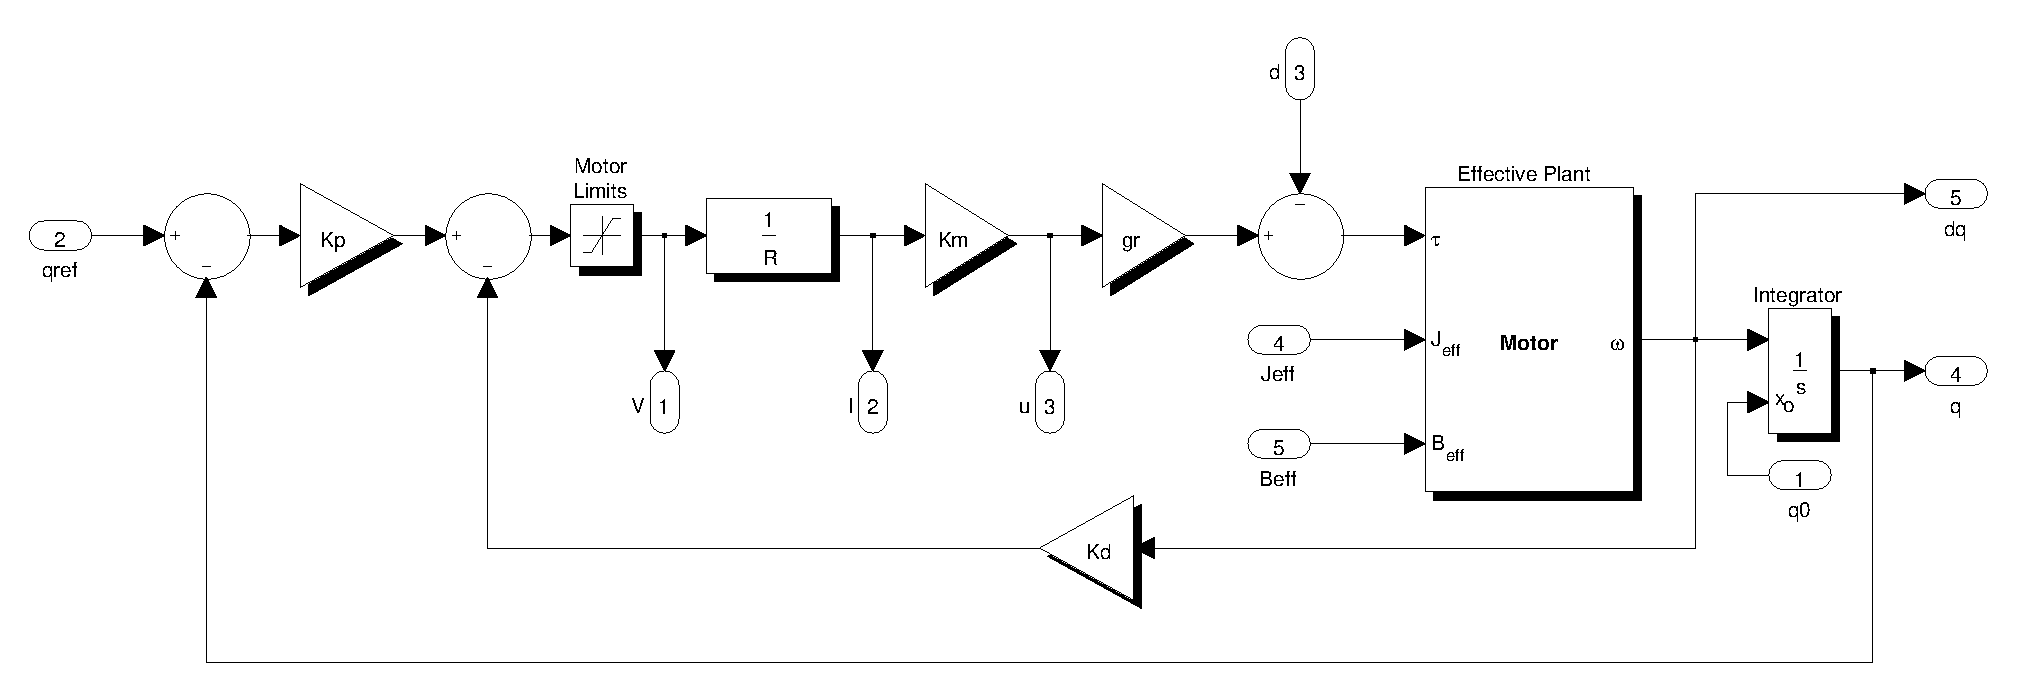
\includegraphics[scale=0.5]{fig/experiments/pdmotorcontroller.eps} 
  	\caption{PD Controller implementation for independent joint control with actuator dynamics. \Incomplete \textbf{- Figure needs to be regenerated to fix the $g_r$ gain block}}
	\label{fig:pdmotorcontroller}
\end{figure}

To improve the estimate of the motor side inertia, $a_{kk}$ is required in (\ref{eq:actdyn6}). The dynamic simulation package used in Section~\ref{sec:simulations_and_results} is based on Mathwork's Simulink environment and uses the SimMechanics toolbox which does not allow the mass matrix $A(\vec{q})$ to be isolated. Therefore, the following algorithm was used to compute the mass matrix and extract the diagonal terms at each time step: 

\begin{algorithm}[H]
 \SetAlgoLined
 Initialization\;
 Set $\vec{q} = \vec{q}_0$, $\vec{\dot q} = \vec{\dot q}_0$, $\vec{\ddot q} = \vec{0}$\;
 \While{1}{
  Compute $\hat{\vtau}$ using RNE with $\vec{\ddot q} = \vec{0}$\;
  \For{$i = 1$ to $n$}{
  Set $\tilde{\vec{g}} = \vec{0}$, $\mathbf{\tilde{\dot{q}}} = \vec{0}$, $\mathbf{\tilde{\ddot{q_i}}} = 1$, $\mathbf{\tilde{\ddot{q_j}}} = 0$ $[j \ne i]$\;
  Compute $\tilde{\vtau}$ using RNE\;
  Form $i$-th column: $A(\vec{q})_{i} = \tilde{\vtau} - \hat{\vtau}$
  }
  Combine columns to form $A(\vec{q})$\;
  Select diagonal elements of $A(\vec{q})$\;
 }
 \caption{Computing mass matrix diagonal terms with RNE algorithm}
 \label{alg:massdiag}
\end{algorithm}

% section actuator_model (end)

\section{HIL Architecture} % (fold)
\label{sec:hil_architecture}
The architecture used to control the physical 14 DOF bipedal robot is presented in this section. In general, controlling DC motors requires a controller (to host the control algorithm) and a driver (typically serves as a power amplifier). The controller outputs a low voltage control signal which is amplified by the driver and applied to the terminals of the motor. Encoders are used to sense the rotor position information and passed back to the controller for closed loop  control. 

The physical hardware developed in Chapter~\ref{cha:design} is treated as the plant. Using Quanser's QUARC toolbox, control algorithms developed in the Simulink environment can be compiled for a variety of target platforms ranging from embedded microcontrollers to standard PC. This allows the use of a shared codebase for simulation and for the physical hardware. The control algorithms used for the biped are compiled and executed on a PC which communicates with the physical hardware through a data acquisition (DAQ) board. A separate and dedicated voltage amplifier is used to drive the DC motors from a low voltage analog control signal (labeled ``amplifier command'' on Figure~\ref{fig:hilarch}) from the controller via the DAQ. 

\begin{figure}[!h]
	\centering
    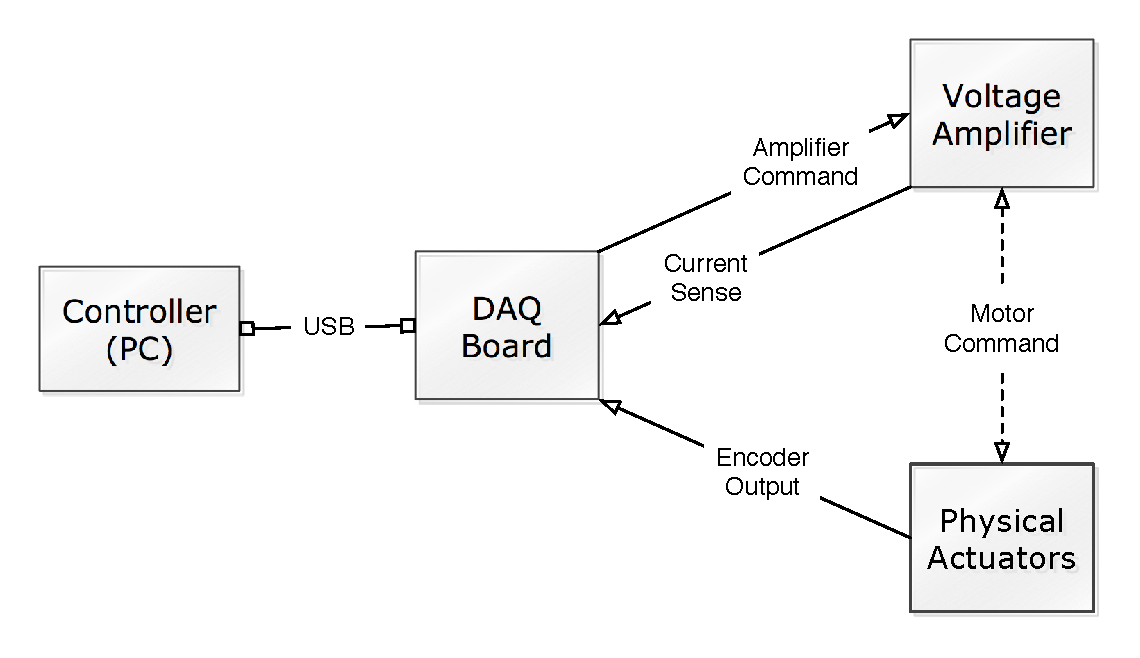
\includegraphics[scale=0.65]{fig/experiments/hilarchitecture.eps} 
  	\caption{Hardware architecture used to control the physical 14 DOF bipedal robot.}
	\label{fig:hilarch}
\end{figure}

The actuator subassemblies selected in Section~\ref{sub:final_configurations} were preassembled with incremental optical encoders mounted to the motor side. These encoders output digital signals on two channels for an indication and control of the motor shaft position and direction.  These digital signals are passed back to the controller running on the PC via the DAQ. Using quadrature decoding, the motor angle $\Theta _m$ and velocity $\dot{\Theta}_m$ can be retrieved from the encoder output in degrees: 

\begin{equation}
	{\Theta _m} = \frac{{360}}{{n \cdot l}} \cdot Encoder_{output}
\end{equation}

Where $n = 4$ for quadrature (4X) decoding and $l$ is the lines per revolution specified from the encoder manufacturer. Using the relationship between the motor variables and the joint variables in (\ref{eq:actdyn2}), an estimate of the $k$-th link side angle (at the output of the gearhead) can be obtained: 

\begin{equation}
	{q_k} = \frac{{360}}{{4 \cdot l \cdot {g_{{r_k}}}}} \cdot Encode{r_k}
	\label{eq:quadrature}
\end{equation}

This is only an estimate of the joint angle since there are drivetrain losses (i.e. in the gearhead) which are ignored by an encoder mounted to the motor side. 

\subsection{Parallel Models} % (fold)
\label{sub:parallel_models}

The ability to develop a single controller and target either a simulation environment or the physical hardware is extremely useful. Using the Quanser's QUARC toolbox, a Q8-USB (DAQ) board and a VoltPAQ (voltage amplifier), the control algorithms were redeveloped as parallel models capable of switching target platforms (shown in Figure~\ref{fig:parallelmodels}).

\begin{figure}[!t]
	\centering
    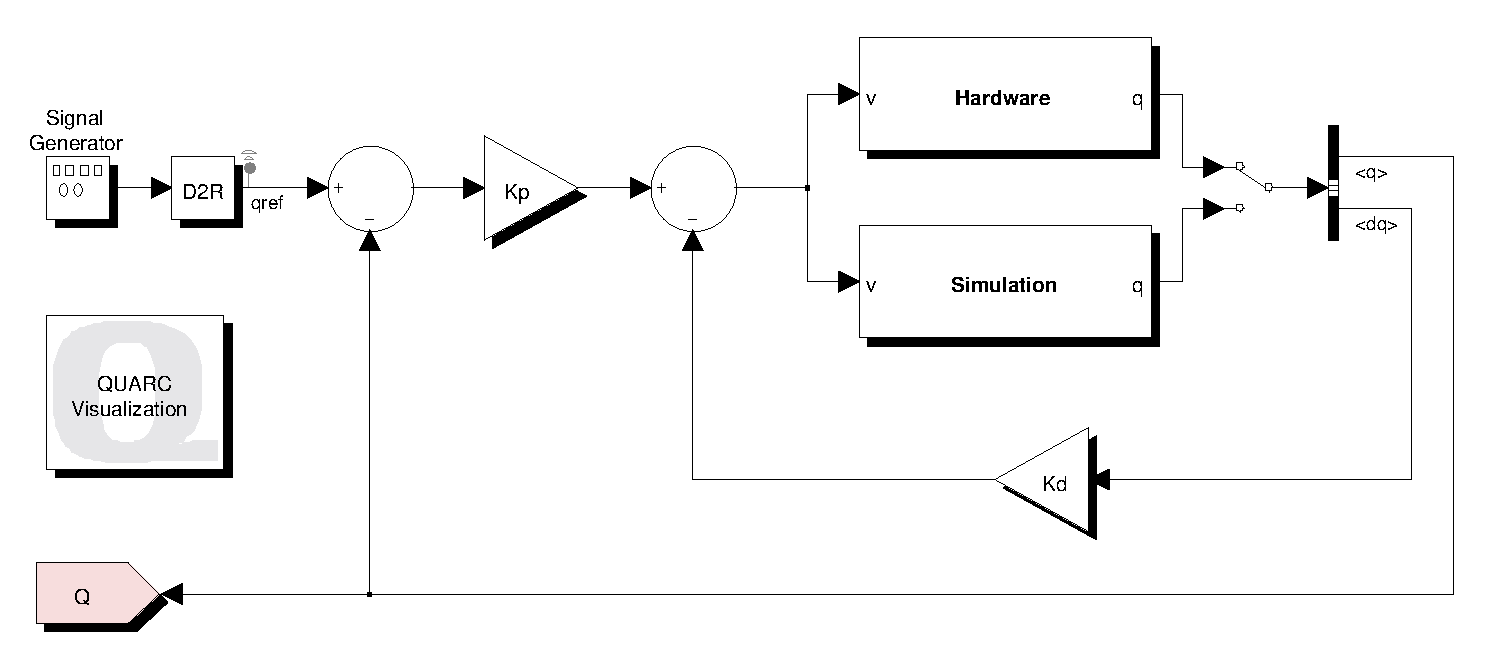
\includegraphics[scale=0.6]{fig/experiments/parallelmodels.eps} 
  	\caption{Parallel models designed to target either simulations or physical hardware with the same controller.}
	\label{fig:parallelmodels}
\end{figure}

\begin{figure}[!b]
	\centering
    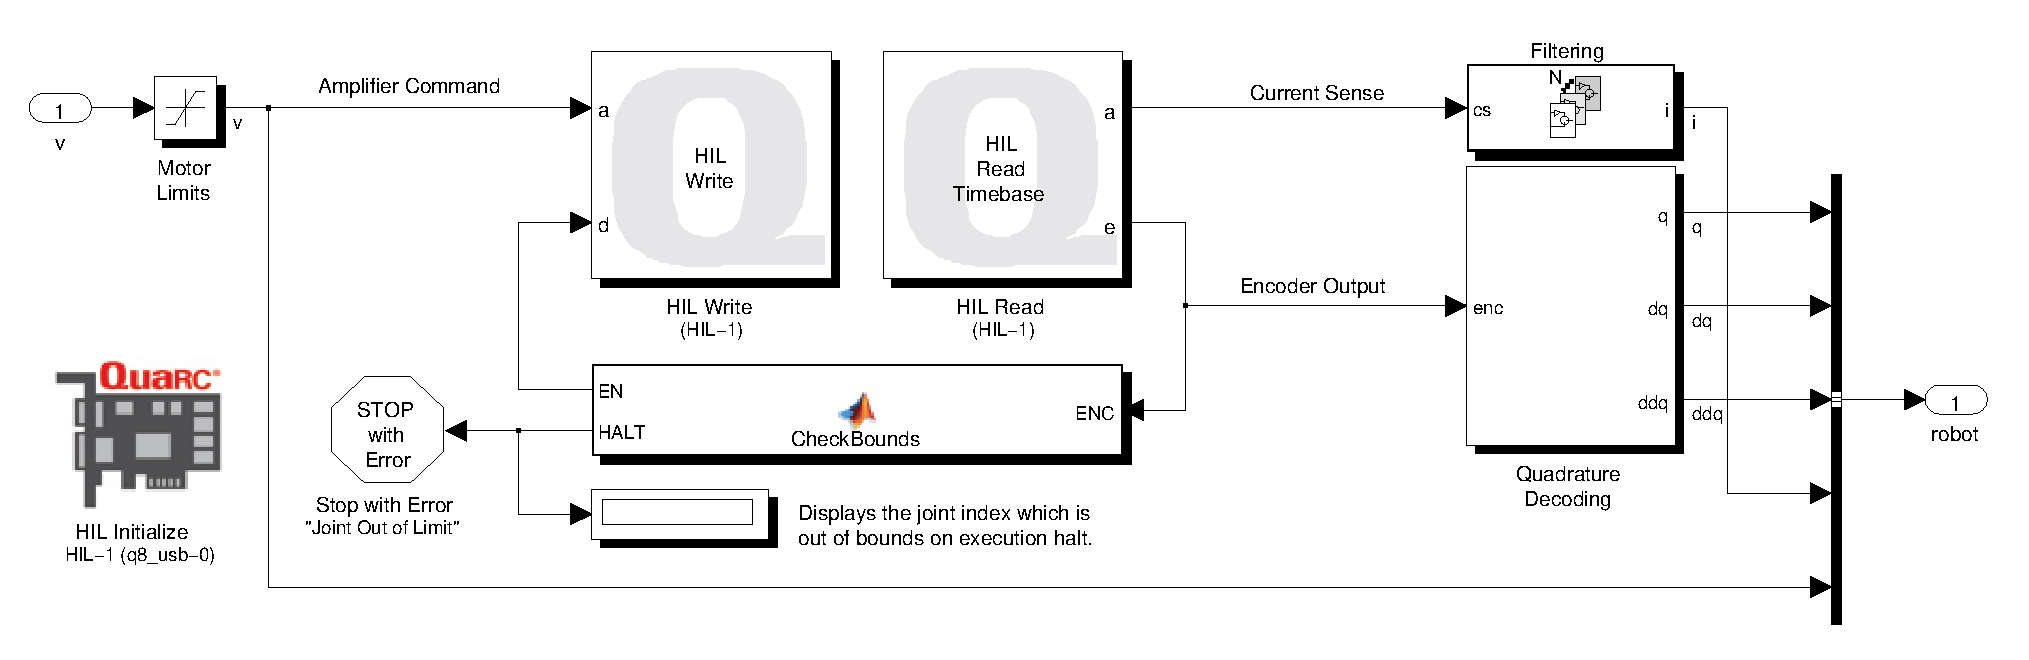
\includegraphics[scale=0.45]{fig/experiments/hilmodel.eps} 
  	\caption{HIL subsystem from Figure~\ref{fig:parallelmodels} used to target physical hardware with voltage control signal.}
	\label{fig:hilmodel}
\end{figure}

In the physical environment mode shown in Figure~\ref{fig:hilmodel}, the hardware target subsystem is initialized to interface with the Q8-USB DAQ board. The control algorithm running on the PC communicates with the physical hardware using ``HIL Read'' and ``HIL Write'' blocks which communicate with the DAQ over USB. The PD controller output is an analog signal corresponding to the desired voltage at the motor terminals (amplifier command). The DAQ also reads the raw digital signals from the motor side encoders. The VoltPAQ voltage amplifier also provides the ability to read the current in the armature circuit ($i_a$) of the DC motor. This value is passed back to the controller through the DAQ using an analog channel. Due to the noise in the current sensor, a low pass filter is used to produce a cleaner signal. The quadrature decoding formula (\ref{eq:quadrature}) is used to obtain the joint angle for the closed loop feedback. The link side angle information is also used to determine whether a joint is out of its limits. The controller detects and sends a ``shut down'' command to the amplifier channel if it is. 

In the simulated environment mode, the controllers were reformulated to use the voltage signal as the control input. The actuator dynamics were incorporated into the simulation using the independent joint control formulation presented in (\ref{eq:actdyn7}). The simulation target subsystem shown in Figure~\ref{fig:simmodel} computes the effective motor inertia and damping seen by the joint using Algorithm~\ref{alg:massdiag}. The link side joint angle, velocity and accelerations are used with inverse dynamics to compute the link side torque which is treated as a disturbance to the system. 

\begin{figure}[!h]
	\centering
    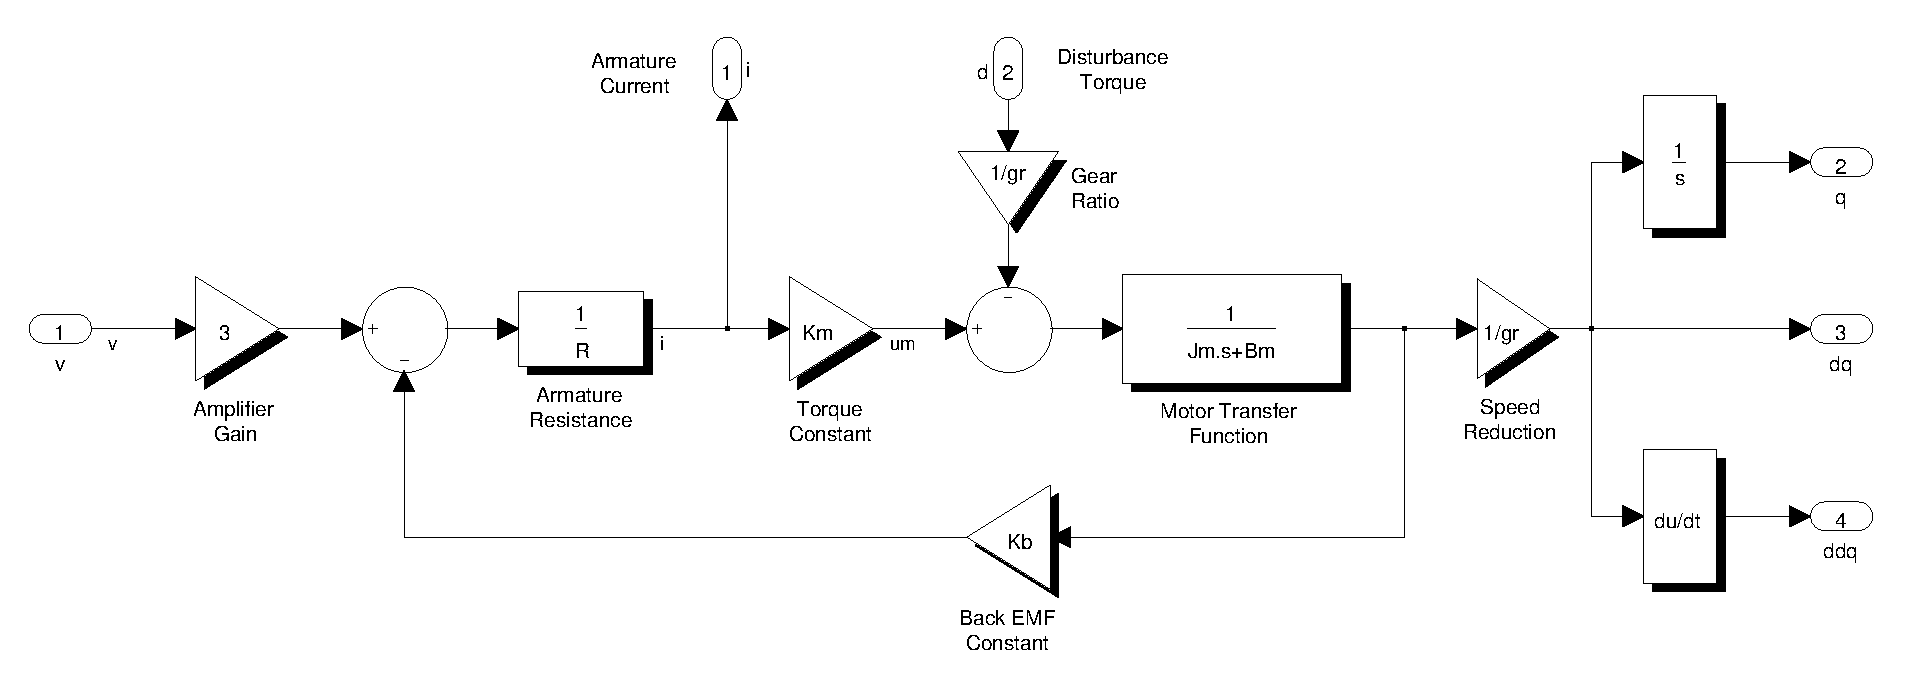
\includegraphics[scale=0.55]{fig/experiments/simmodel.eps} 
  	\caption{Subsystem from Figure~\ref{fig:parallelmodels} used to target the simulated environment with voltage control signal. \Incomplete \textbf{- Figure needs to be regenerated to fix the $g_r$ gain block}}
	\label{fig:simmodel}
\end{figure}


% subsection parallel_models (end)

% section hil_architecture (end)

\section{Single DOF Validation} % (fold)
\label{sec:1dof_validation}
This section describes the experiments validating the simulation models for 1 DOF controllers using the HIL environment. 

\subsection{Joint Tracking} % (fold)
\label{sub:joint_tracking}
The parallel model for targetting the simulation environment and physical hardware was used to tune the PD controller gains for a single joint of the bipedal robot. By using the shared controller architecture, gains were tuned to improve tracking performance in the simulation environment and then immediately verified on the physical hardware. The experimental results presented in this section show the results of the joint tracking a sine wave at 0.5 Hz in hardware and simulation. 

%The same controller gains were used on the physical hardware and the tracking performance is almost identical to the simulated case. The tracking results shown in Figure~\ref{fig:hipyawtracking} validate the simulation model for the hip yaw joint. 

\begin{figure}[!h]
	\begin{center}
	\subfigure{\includegraphics[scale=0.45]{fig/experiments/hipyawtrackingsim.eps}}
	\subfigure{\includegraphics[scale=0.45]{fig/experiments/hipyawtrackinghil.eps}}
	\end{center}
  	\caption{Hip yaw joint tracking results for simulation and hardware.}
	\label{fig:hipyawtracking}
\end{figure} 

% \begin{figure}[!h]
% 	\begin{center}
% 	\subfigure{\includegraphics[scale=0.45]{fig/experiments/hipyawvoltages.eps}}
% 	\subfigure{\includegraphics[scale=0.45]{fig/experiments/hipyawcurrents.eps}}
% 	\end{center}
%   	\caption{Hip yaw joint voltage and current in simulation and hardware.}
% 	\label{fig:hipyawelectrical}
% \end{figure} 

\begin{figure}[!h]
	\begin{center}
	\subfigure{\includegraphics[scale=0.45]{fig/experiments/hippitchtrackingsim.eps}}
	\subfigure{\includegraphics[scale=0.45]{fig/experiments/hippitchtrackinghil.eps}}
	\end{center}
  	\caption{Hip pitch joint tracking results for simulation and hardware.}
	\label{fig:hippitchtracking}
\end{figure} 

% \begin{figure}[!h]
% 	\begin{center}
% 	\subfigure{\includegraphics[scale=0.45]{fig/experiments/hippitchvoltages.eps}}
% 	\subfigure{\includegraphics[scale=0.45]{fig/experiments/hippitchcurrents.eps}}
% 	\end{center}
%   	\caption{Hip pitch joint voltage and current in simulation and hardware.}
% 	\label{fig:hippitchelectrical}
% \end{figure} 

\begin{figure}[!h]
	\begin{center}
	\subfigure{\includegraphics[scale=0.45]{fig/experiments/kneepitchtrackingsim.eps}}
	\subfigure{\includegraphics[scale=0.45]{fig/experiments/kneepitchtrackinghil.eps}}
	\end{center}
  	\caption{Knee pitch joint tracking results for simulation and hardware.}
	\label{fig:kneepitchtracking}
\end{figure} 

% \begin{figure}[!h]
% 	\begin{center}
% 	\subfigure{\includegraphics[scale=0.45]{fig/experiments/kneepitchvoltages.eps}}
% 	\subfigure{\includegraphics[scale=0.45]{fig/experiments/kneepitchcurrents.eps}}
% 	\end{center}
%   	\caption{Knee pitch joint voltage and current in simulation and hardware.}
% 	\label{fig:kneepitchelectrical}
% \end{figure} 
 
% subsection joint_tracking (end)

\cleardoublepage
% section 1dof_results (end)

\section{Motion Control Validation} % (fold)
\label{sec:motion_control_validation}
\Incomplete

\subsection{Planar Motion Control} % (fold)
\label{sub:planar_motion_control}

\subsubsection{Knee Bending Motion} % (fold)
\label{ssub:knee_bending_motion}
\begin{figure}[!h]
	\centering
    \includegraphics[scale=0.22]{fig/experiments/kneebendframes.png} 
  	\caption{Captured frames during knee bending experiment in simulation and physical hardware.}
	\label{fig:kneebendframes}
\end{figure}

\begin{figure}[!h]
	\begin{center}
	\subfigure{\includegraphics[scale=0.45]{fig/experiments/simkneebendp.eps}}
	\subfigure{\includegraphics[scale=0.45]{fig/experiments/hilkneebendp.eps}}
	\end{center}
  	\caption{Task space trajectory tracking for bending the knee and raising the leg in simulation and hardware.}
	\label{fig:kneebendp}
\end{figure} 

\cleardoublepage
% subsubsection knee_bending_motion (end)

\subsubsection{Swing Foot Motion} % (fold)
\label{ssub:swing_foot_motion}

\begin{figure}[!h]
	\centering
    \includegraphics[scale=0.145]{fig/experiments/swingmotionframes.png} 
  	\caption{Captured frames during swing foot motion experiment in simulation and physical hardware.}
	\label{fig:swingmotionframes}
\end{figure}

\begin{figure}[!h]
	\begin{center}
	\subfigure{\includegraphics[scale=0.45]{fig/experiments/simswingfootp.eps}}
	\subfigure{\includegraphics[scale=0.45]{fig/experiments/hilswingfootp.eps}}
	\end{center}
  	\caption{Task space trajectory tracking for swing foot motion in simulation and hardware.}
	\label{fig:swingfootp}
\end{figure} 

\begin{figure}[!h]
	\begin{center}
	\subfigure{\includegraphics[scale=0.45]{fig/experiments/simswingfootq.eps}}
	\subfigure{\includegraphics[scale=0.45]{fig/experiments/hilswingfootq.eps}}
	\end{center}
  	\caption{Joint space tracking of generated trajectories from higher level control during swing foot motion.}
	\label{fig:swingfootq}
\end{figure} 
\cleardoublepage
% subsubsection swing_foot_motion (end)





% subsection planar_motion_control (end)

\subsection{Whole Body Motion Control} % (fold)
\label{sub:whole_body_motion_control}
\Incomplete
% subsection whole_body_motion_control (end)

% section motion_control_results (end)

\section{Summary} % (fold)
\label{sec:experiments_summary}
Validating control algorithms on physical hardware is important due to modeling imperfections in the simulation environment. The physical 14 DOF bipedal robot developed in earlier chapters was used for experimental validation through HIL testing. 

For the physical hardware, DC motors are controlled by a voltage signal $v_m$. A second order system was used to model the actuator dynamics and reformulate the existing controllers which controlled the link side torques $\tau _k$. Independent joint control decouples each joint for individual control. Since this approach does not account for the coupled dynamics of the overall system, the link side torques are treated as a disturbance to the actuator dynamics model. The effective motor inertia is reformulated to include the link inertia seen by the joint. A generic RNE-based algorithm was used to extract the mass matrix of the system at every time step to compute the effective motor inertia.

The HIL architecture was developed using Quanser's QUARC toolbox, DAQ board and a voltage amplifier. The controller code developed in Simulink was targetted to execute on the PC. The DAQ board allowed the PC-based controller to communicate with the physical hardware through analog and digital I/O. Quadrature decoding was on the encoder output to obtain the link side joint angles on physical hardware for closed loop feedback control. Parallel simulation models were developed for experimental validation to target the physical hardware or the simulated actuator dynamics. 

The single DOF simulations were demonstrated on physical hardware. The simulated environment was used to tune the PD gains for the physical hardware. It was shown that tracking performance of the PD controller was identical in both environments.  

\Incomplete
% section discussion (end)

% chapter experiments (end)
    \chapter{Conclusions} % (fold)
\label{cha:conclusion}
\ifthenelse{\boolean{VoidIncomplete}}{\Incomplete}{

Lorem ipsum dolor sit amet, consectetur adipisicing elit, sed do eiusmod
tempor incididunt ut labore et dolore magna aliqua. Ut enim ad minim veniam,
quis nostrud exercitation ullamco laboris nisi ut aliquip ex ea commodo
consequat. Duis aute irure dolor in reprehenderit in voluptate velit esse
cillum dolore eu fugiat nulla pariatur. Excepteur sint occaecat cupidatat non
proident, sunt in culpa qui officia deserunt mollit anim id est laborum.

\section{Future Work} % (fold)
\label{sec:future_work}
Lorem ipsum dolor sit amet, consectetur adipisicing elit, sed do eiusmod
tempor incididunt ut labore et dolore magna aliqua. Ut enim ad minim veniam,
quis nostrud exercitation ullamco laboris nisi ut aliquip ex ea commodo
consequat. Duis aute irure dolor in reprehenderit in voluptate velit esse
cillum dolore eu fugiat nulla pariatur. Excepteur sint occaecat cupidatat non
proident, sunt in culpa qui officia deserunt mollit anim id est laborum.

% section future_work (end)
}
% chapter conclusion (end)

    % B A C K   M A T T E R
    %======================================================================
%   B A C K  M A T T E R
%======================================================================


% B I B L I O G R A P H Y
% -----------------------
\bibliographystyle{plain}
\cleardoublepage 
\phantomsection

\renewcommand*{\bibname}{References} % Use "References" instead of "Bibliography"
\addcontentsline{toc}{chapter}{\textbf{References}} % Add the References to the Table of Contents

\bibliography{bib/masc-thesis}
\nocite{*}


% A P P E N D I C E S
% -------------------
% \appendix
% \chapter*{Appendices} % Add a title page before the appendices and a line in the Table of Contents
% \addcontentsline{toc}{chapter}{Appendices}

% %======================================================================
\chapter[PDF Plots From Matlab]{Matlab Code for Making a PDF Plot}
%======================================================================
\label{AppendixA}

\section{Using the GUI}
Properties of Matab plots can be adjusted from the plot window via a graphical interface. Under the Desktop menu in the Figure window, select the Property Editor. You may also want to check the Plot Browser and Figure Palette for more tools. To adjust properties of the axes, look under the Edit menu and select Axes Properties.

To set the figure size and to save as PDF or other file formats, click the Export Setup button in the figure Property Editor.

\section{From the Command Line} 
All figure properties can also be manipulated from the command line. Here's an example: 

\begin{verbatim}
	x=[0:0.1:pi];
	hold on % Plot multiple traces on one figure
	plot(x,sin(x))
	plot(x,cos(x),'--r')
	plot(x,tan(x),'.-g')
	title('Some Trig Functions Over 0 to \pi') % Note LaTeX markup!
	legend('{\it sin}(x)','{\it cos}(x)','{\it tan}(x)')
	hold off
	set(gca,'Ylim',[-3 3]) % Adjust Y limits of "current axes"
	set(gcf,'Units','inches') % Set figure size units of "current figure"
	set(gcf,'Position',[0,0,6,4]) % Set figure width (6 in.) and height (4 in.)
	cd n:\thesis\plots % Select where to save
	print -dpdf plot.pdf % Save as PDF
\end{verbatim}


\end{document}

\bye
